\NeedsTeXFormat{LaTeX2e}
\documentclass[a4paper,10pt,bibtotoc,twoside,openright,pointlessnumbers,normalheadings,DIV=9
%,draft
]{scrbook}
\KOMAoptions{DIV=last}


\pagestyle{headings}
\usepackage{ngerman}
\usepackage[utf8]{inputenc}
\usepackage[T1]{fontenc}
\renewcommand{\sfdefault}{phv}
%\renewcommand{\rmdefault}{phv}
\renewcommand{\ttdefault}{pcr}
\usepackage{graphicx}
\usepackage{verbatim}
\usepackage{tabularx}
\usepackage{subfigure}
\usepackage{url}
\usepackage{color}
\usepackage{amssymb}
\usepackage{setspace}
\usepackage{listings}
\lstset{language=Java,
  showstringspaces=false,
  frame=single,
  numbers=left,
  basicstyle=\ttfamily,
  numberstyle=\tiny}

% hier Namen etc. einsetzen
\newcommand{\fullname}{Stefan Langenmaier}
\newcommand{\email}{stefan.langenmaier@uni-ulm.de}
\newcommand{\titel}{Implementierung und Optimierung eines relationalen Schlussfolgerungssystems}
%\newcommand{\titel}{Titel der Arbeit}
\newcommand{\jahr}{2009}
\newcommand{\matnr}{575546}
\newcommand{\gutachterA}{Prof.~Dr.~Friedrich von Henke}
\newcommand{\gutachterB}{Dr.~Thorsten Liebig}
\newcommand{\betreuer}{Dr.~Thorsten Liebig}
% hier richtige Fakultät auswählen
\newcommand{\fakultaet}{Ingenieurwissenschaften\\und Informatik}
%\newcommand{\fakultaet}{Mathematik und\\Wirtschaftswissenschaften}
%\newcommand{\fakultaet}{Naturwissenschaften}
%\newcommand{\fakultaet}{Medizin}
% nun noch unten das Institut einsetzen
\newcommand{\institut}{Institut für Künstliche Intelligenz}

%color in tables
\usepackage{colortbl}
\definecolor{Gray}{rgb}{0.80784, 0.86667, 0.90196} %dunkelblau
\definecolor{Lightgray}{rgb}{0.9176, 0.95, 0.95686} %hellblau
\definecolor{Akzent}{rgb}{0.6627, 0.63529, 0.55294} %akzentfarbe
\setlength{\arrayrulewidth}{0.1pt}

\clubpenalty10000
\widowpenalty10000

\setlength{\parindent}{0pt}
\setlength{\parskip}{1.4ex plus 0.35ex minus 0.3ex}

% Tiefe, bis zu der Überschriften in das Inhaltsverzeichnis kommen
\setcounter{tocdepth}{3}

\pdfinfo{
  /Author (\fullname)
  /Title (\titel)
  /Producer     (pdfeTex 3.1415926-1.40.9-2.2)
  /Keywords ()
}

\usepackage{hyperref}
\hypersetup{
pdftitle=\titel,
pdfauthor=\fullname,
pdfsubject={Diplomarbeit},
pdfproducer={pdfeTex 3.1415926-1.40.9-2.2},
colorlinks=false,
pdfborder=0 0 0	% keine Box um die Links!
}

\usepackage{tikz}
\usetikzlibrary{positioning,shapes,shadows,arrows}

 
%Trennungsregeln
\hyphenation{Sil-ben-trenn-ung}

\begin{document}
\frontmatter

% Titelseite
\thispagestyle{empty}
\begin{addmargin*}[4mm]{-32mm}


\includegraphics[height=1.8cm]{images/unilogo_bild}
\hfill

\includegraphics[height=1.8cm]{images/unilogo_wort}\\[1em]

{\footnotesize
{\bfseries Universität Ulm} \textbar ~89069 Ulm \textbar ~Germany
\hspace*{60mm}\parbox[t]{48mm}{\bfseries Fakultät für\\
\fakultaet\\
\mdseries \institut}\\[2cm]

\parbox{140mm}{\bfseries \huge \titel}\\[0.5em]
{\footnotesize Diplomarbeit an der Universität Ulm}\\[3em]

{\footnotesize \bfseries Vorgelegt von:}\\
{\footnotesize \fullname\\\email}\\[2em]
{\footnotesize \bfseries Gutachter:}\\                     
{\footnotesize\gutachterA\\
\gutachterB}\\[2em]
%{\footnotesize \bfseries Betreuer:}\\ 
%{\footnotesize\betreuer}\\\\
{\footnotesize\jahr}
}
\end{addmargin*}


% Impressum
\clearpage
\thispagestyle{empty}
{ \small
  \flushleft
  Fassung, \today \\\vfill
  \copyright~\jahr~\fullname\\[0.5em]
% Falls keine Lizenz gewünscht wird bitte den folgenden Text entfernen.
% Die Lizenz erlaubt es zu nichtkommerziellen Zwecken die Arbeit zu
% vervielfältigen und Kopien zu machen. Dabei muss aber immer der Autor
% angegeben werden. Eine kommerzielle Verwertung ist für den Autor
% weiter möglich.
%This work is licensed under the Creative Commons
% Attribution-NonCommercial-ShareAlike 3.0 License. To view a copy of this license, visit http://creativecommons.org/licenses/by-nc-sa/3.0/de/ or send a letter to Creative Commons, 543 Howard Street, 5th Floor, San Francisco, California, 94105, USA. \\

  Satz: PDF-\LaTeXe
}


% ab hier Zeilenabstand 1,4 fach 10pt/14pt
\setstretch{1.4}

\tableofcontents



\mainmatter

\section*{Zusammenfassung}
Diese Arbeit beschäftigt sich mit der Implementierung und Optimierung eines relationalen Schlussfolgerers. Dieser Schlussfolgerer arbeitet dabei auf dem OWL2 RL Profil, das Ende Oktober 2009 vom W3C \cite{OWL2Profiles} veröffentlicht wurde. Dieser \emph{technical report} stellt eine Spezifikation der Semantik und der möglichen Schlussfolgerungsregeln in einer Ontologie dar. Die Veröffentlichung der Spezifikation des W3C ist frei zugänglich und kompatibel zur Vorgängerversion OWL1 \cite{OWL1}, sie steht damit einer breiten Basis von Anwendungen und Anwendern zur Verfügung. Allerdings sind konkrete Umsetzungen von Software für OWL2 auf Grund seiner aktuellen Natur noch nicht vorhanden bzw. im Moment in der Entwicklung. In dieser Arbeit wird daher auf teilweise noch experimenteller Software, wie z.B. der OWLAPI v3 \cite{OWLAPI}, aufgesetzt. Dies ist nötig, um für die Zukunft eine aktuelle Schnittstelle für Ontologien zur Verfügung zu stellen.

Einige Prinzipien, wie ein solcher Reasoner implementiert werden kann, basieren dabei in einigen Teilen auf der Diplomarbeit \emph{Speicherung und Abfrage großer Ontologien in deduktiven Datenbanken} aus dem Oktober 2003 von Timo Weithöhner. Sie ist damit auch eine Fortsetzung der Entwicklung des U2R2 (Uni Ulm Relational Reasoner). Es wird daher angenommen, das der Leser zumindest mit den Erkenntnissen und Ergebnissen dieser Arbeit vertraut ist.

Es wird im folgenden ein relationaler Reasoner mit \emph{forward-chaining} und \emph{direct materialisation} entwickelt. Relational steht dabei dafür, das die Ergebnisse und Fakten der Ontologien in Relationen in einer Datenbank abgespeichert werden. Forward-chaining bedeutet, dass aus existierenden Fakten durch Anwendung von Schlussfolgerungsregeln neue Fakten erzeugen werden und darauf wieder die Schlussfolgerungsregeln angewendet werden. Dies geschieht bis keine neuen Fakten mehr erzeugt werden können. Direct-materialisation steht dafür, dass alle erzeugten Fakten abgespeichert werden und somit zur Anfragezeit alle möglichen Antworten schon vorliegen und dann nur noch ausgegeben werden müssen.

Durch diese Eigenschaften ist es einerseits möglich große Ontologien zu laden und sie nicht vollständig im Arbeitsspeicher halten zu müssen, indem man sie im Sekundärspeicher durch ein Datenbanksystem verwaltet. Andererseits wird durch den direct-materialisation Ansatz der Fokus auf die Beantwortung von Fragen an die Ontologie gelenkt. Durch eine Vorberechnung ist es sehr schnell möglich darauf zu antworten. Das ist auch der angenommene Anwendungsfall für u2r3. Die Anzahl der Anfragen überwiegt bei weitem  die Zeit für die Vorberechnung. Die Zeit für die Beantwortung von Anfragen ist wichtiger niedrig zu halten, als die Zeit für die Vorberechnung.

Damit sollte die grundlegende Arbeitsweise aufgezeigt sein und der Leser sollte einen Überblick zum Gebiet der Implementierung haben.

%Kapitel Motivation
    * Was ist Sinn und Zweck dieser Arbeit?
    * Engültige Fragen
          o Lohnt sich der Speicher/Vorbereitungszeit-Tradoff gegenüber der Anfragezeit?
          o Wie können Änderungen effizient realisiert werden? 
    * Was wird hier behandelt?
          o Wo ist das OWL2 RL Fragment einzuordnen?
          o Wie ist OWL2 aufgebaut?
          o Was sind andere Profile
          o Was sind ihre Unterschiede
          o Was sind ihre Eigenschaften. 

%Kapitel Grundlagen
\chapter{Grundlagen \& Vorarbeiten}
\label{kapitel-grundlagen}
Im folgenden werden Begriffe aus dem Bereich Wissenmodellierung und Wissensrepräsentation näher erklärt, da diese die formale Grundlage der Arbeit bilden.

Dazu gehören Ontologien, für was sie stehen und die Beschreibung des OWL2 RL Fragments. Das Verständnis für einen Schlussfolgerer, sowie einige Hintergründe für die Umsetzungen von Ontologien in Datenbanken.

Außerdem werden auch einige Begriffe angesprochen die sonst für die Arbeit wichtig sind, aber nicht intuitiv zu erschließen sind. Dazu gehören unter anderem Regeln und Relationen.

\section{Ontologien}

Ontologien sind nach einem Formalismus erzeugte Beschreibungen eines Teilausschnittes der Welt, die formal ableitbare Aussagen ermöglichen. Sie haben damit eine entfernte Beziehung zu Datenbanken, die z.B. nach einem ER-Modell entwickelt wurden. Ontologien enthalten dabei die Struktur und Beziehung der Daten, sowie die Daten selbst. Anders als in einem ER-Modell sind aber die Daten und die Struktur nicht strikt von einander getrennt. Der Formalismus auf dem eine Ontologie aufsetzt ist im Rahmen der W3C Semantic Web Initiative stark von Logik geprägt. \cite{Hesse2002}

\subsection{Unterschied zu relationaler Datenbank}

Beim Abspeichern einer Ontologie in einer relationalen Datenbank sind zwei konzpetionelle Dinge zu beachten. In einer Ontologie gilt die \emph{unique name assumption}, das bedeutet das in der Ontologie verwendete Namen zum identifizieren von Entitäten eindeutig sind und sicher immer auf die selbe Entität beziehen. In OWL gilt das nur zum Teil, da es hier möglich ist auszudrücken, das zwei Namen identisch oder verschieden sind\cite{OWL1}\footnote{Die Ausdrücke sind \texttt{owl:sameAs} und \texttt{owl:differentFrom}.}. In einer Relation ist das nicht zwingend vorausgesetzt. Nur wenn Spalten als Schlüssel oder als \emph{unique} deklariert werden, wird sichergestellt das Namen eindeutig sind.
Der zweite Unterschied besteht darin, wie man über die Daten schließt. In einer Datenbank geht man davon aus, das man die komplette Welt modelliert hat und alle Fakten vorhanden sind. Kann etwas nicht gefunden werden, ist es nicht Teil des Modells und damit falsch. In einer Ontologie werden Fakten, die nicht vorhanden sind als unbekannt eingestuft. Sie sind damit weder wahr noch falsch. Datenbanken verwenden damit eine sog. \emph{closed-world assumption} (CWA) und Ontologien eine \emph{open-world assumption} (OWA).

\section{OWL2}
\label{abschnitt-owl2}

\begin{figure}[htb]
	\caption{Adaption des W3 Layercake\cite{W3SWLayerCake}}
	\label{image-w3-layercake}
	\begin{center}
	\scalebox{0.35}{
		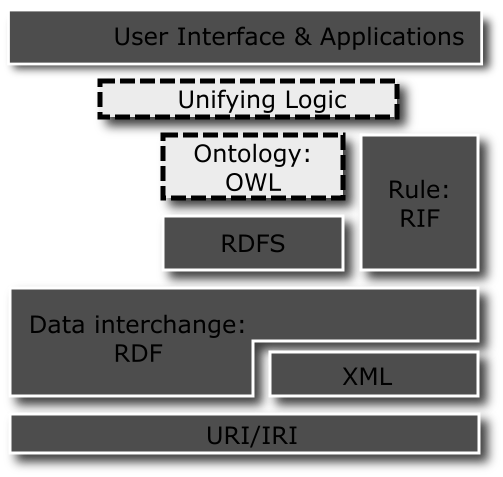
\includegraphics{images/w3-layercake.pdf}
	}
	\end{center}
\end{figure}


Abbildung \ref{image-w3-layercake} zeigt eine Adaption des offizielen W3 OWL Layercake\cite{W3SWLayerCake}. Es wurden alle Teile entfernt, die die Implementierung nicht betreffen. Dabei ist der helle Teil mit einer getrichelten Linie der in der Arbeit verwendete Teil. Der obere Teil ``User Interface \& Applications'' ist die Anwendungsschnittstelle, die z.B. durch die OWLAPI gekapselt wird. Die unteren Blöcke sind Web-Standards auf denen denen aufgebaut wird. Sie spielen in der Arbeit keine Rolle und sind für das Verständnis nicht näher benötigt.Der RIF Abschnitt ist hier erwähnt, weil er eine alternative Regelumsetzung bietet. Dies wird in Abschnitt \ref{abschnitt-rif} näher erläutert.

\begin{figure}[htb]
	\caption{Sprachkomplexitäten}
	\label{image-sprachhierarchie}
	\begin{center}
		\scalebox{0.4}{
			\includegraphics{images/sprachhierarchie.pdf}
		}
	\end{center}
\end{figure}

Die Abbildung \ref{image-sprachhierarchie} gibt einen Einblick in die Verhältnisse der Ausdrucksmächtigkeit, von OWL und wie sie in den größeren Kontext von Logik eingeordnet werden.

\begin{verbatim}
OWL2 TEXT
\end{verbatim}


\section{Sprachkomplexitäten}
Im folgenden werden verschieden Sprachen an Hand ihrer Komplexität kurz gegenüber gestellt, um einen Vergleichsbasis zu haben.

\begin{figure}[htb]
	\caption{OWL Logikeinordnungen, nach einer Vorlage aus \cite{OWLimLayerMap}}
	\label{image-owl-layer-map}
	\begin{center}
	\scalebox{0.35}{
		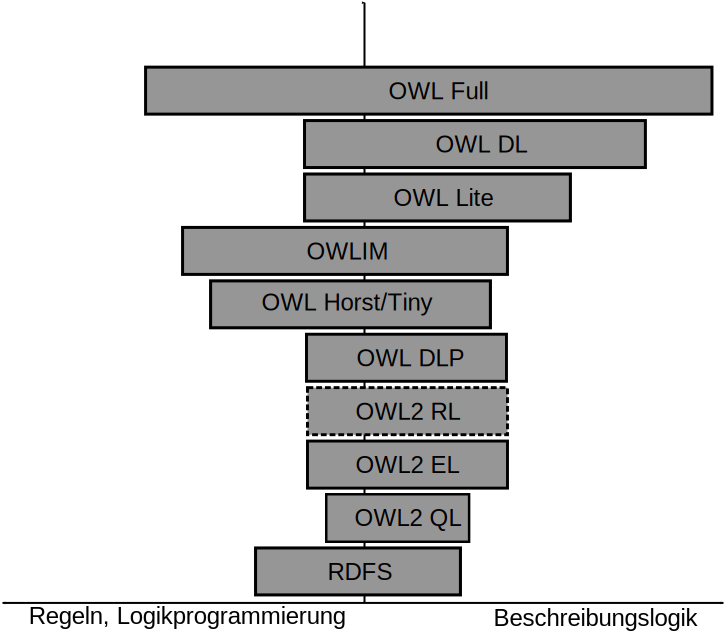
\includegraphics{images/owl-layer-map.pdf}
	}
	\end{center}
\end{figure}
Abbildung \ref{image-owl-layer-map} frei nach der Vorlage aus der OWLim Dokumentation. In dieser Abbildung wird der Einfluss der verschiedenen Semantiken von Logiken dargestellt.

\subsection{Attributive Language}
Die \emph{Attributive Language} ist eine einfache Beschreibungssprache. Sie wird mit $\mathcal{AL}$ abgekürzt und enthält folgende Operatoren für ihre Ausdrucksmöglichkeiten. Sie ist die Grundlage viler Sprachen, wie auch von OWL2.

$\mathcal{AL}$: C,D $\Longrightarrow$ A | $\top$ | $\bot$ | $\lnot$A | C $\land$ D | $\forall$r.C | $\exists$r

Diese attributive language kann durch weitere Operatoren in ihrere Ausdrucksmächtigkeit vergrößert werden. Für die Menge an Möglichkeiten hat sich dabei ein Namensschema herauskristallisiert. Dies ist zwar kein offizielles und eindeutiges Schema, wird aber von vielen Programmen wie z.B. Protégé verwendet.

Bei diesem Namenschema werden an die Buchstaben $\mathcal{AL}$ noch weitere Kürzel angehängt, die für die zusätzlichen Operatoren stehen.
\begin{itemize}
  \item $\mathcal{C}$ für volle Negation (Complement)
  \item (D) für konkrete Domänen\newline
Damit ist der Einsatz von Literalen möglich, z.B. in \emph{datatype properties}, \emph{data values} oder \emph{data types}.
  \item $\mathcal{U}$ Konzeptvereinigung (Union)
  \item $\mathcal{E}$ Existenzquantoren für komplexe Ausdrücke (Exists)\newline
Existenzquantoren sind für alle Arten von Ausdrücken erlaubt.
  \item $\mathcal{N}$ Kardinalitätseinschränkungen
  \item $\mathcal{I}$ Inverse Eigenschaften (Inverse)
  \item $\mathcal{O}$ Aufzählungen von \emph{object values} (Nominals)
  \item $\mathcal{H}$ Hierarchie von Eigenschaften (Role hierarchy)
  \item $\mathcal{F}$ Funktionale Eigenschaften
  \item $\mathcal{S}$ Die Abkürzung für $\mathcal{ALC}$ mit transitiven Eigenschaften
\end{itemize}
\cite{wiki:DescriptionLogic}

\subsection{Komplexität in Form der attributive language}
\begin{itemize}
  \item U2R2 basiert auf der DLP Sprache und ist damit ein Reasoner auf der $\mathcal{ALCHIF}$-Sprache ($\mathcal{SHIF}$). Hier gibt es allerdings Einschränkungen ähnlich wie in OWL2 RL. Es sind nicht, alle Konsturkte an jeder Stelle erlaubt, ansonsten sind Schlussfolgerungen nicht mehr vollständig.
  \item OWL2 basiert auf $\mathcal{ALCROIQ}$ ($\mathcal{SROIQ}$) \cite{Krötzsch2008}
\end{itemize}


\begin{figure}[htb]
	\caption{Sprachkomplexitäten}
	\label{image-sprachkomplexitaeten}
	\begin{center}
		\scalebox{0.4}{
			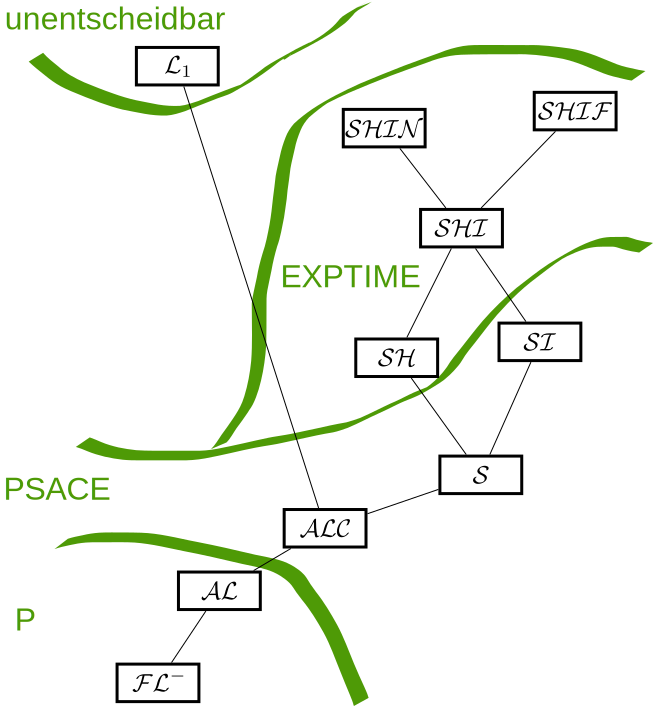
\includegraphics{images/sprachkomplexitaeten-wimo-blatt4.pdf}
		}
	\end{center}
\end{figure}
Die Abbildung \ref{image-sprachkomplexitaeten} ist frei nach der Vorlesung/Übung Wissensmodellierung \cite{vonHenke2009} modelliert. Es wird das ``computational cliff'' dargestellt. Man kann erkennen welche Sprachen welche Berechnungskomplexitäten haben

\begin{table}
	\caption{Sprachkomplexitäten}
	\label{table-sprachkomplexitaeten}
%	\rowcolors{3}{white}{lightgray}
	
	\scalebox{0.74}{
		\renewcommand{\arraystretch}{1.2}
		\begin{tabular}{|M{2cm}|p{2cm}|p{3cm}|p{3cm}|p{3cm}|p{3cm}|}
		\hline
		\rr Sprache & \rr Schluss\-folger\-ungs\-problem & \rr Komplexität der Taxonmie & \rr Daten\-komplexität & \rr Abfrage Komplexität & \rr Kombinierte Komplexität \tn
		\hline
		\hline
		\multirow{3}{*}{OWL-DL} & Ableitung & NEXPTIME-vollständig & Offen & Nicht anwendbar & NEXPTIME-vollständig \\ 
		\cline{2-6}
								& Abfragen & Offen & Offen & Offen & Offen \\
		\hline
		\multirow{3}{*}{DLP} & Ableitung & In EXPTIME & PTIME-vollständig & Nicht anwendbar & In EXPTIME \\
							\cline{2-6}
							& Abfragen & In EXPTIME & PTIME-vollständig & In EXPTIME & In EXPTIME \\
		\hline
		\rr \multirow{4}{2cm}{OWL2 Direct Semantics} & Ableitung & 2NEXPTIME-vollständig & entscheidbar, aber Komplexität offen & Nicht anwendbar & 2NEXPTIME \\
			\cline{2-6}
			& Abfragen & Entscheidbarkeit offen & Entscheidbarkeit offen & Entscheidbarkeit offen & Entscheidbarkeit offen \\
		\hline
		\multirow{3}{*}{OWL2 EL} & Ableitung & PTIME-vollständig & PTIME-vollständig & Nicht anwendbar & PTIME-vollständig \\
			\cline{2-6}
			& Abfragen & PTIME-vollständig & PTIME-vollständig & NP-vollständig & PSPACE-vollständig \\
		\hline
		\multirow{3}{*}{OWL2 QL} & Ableitung & NLogSpace-vollständig & In AC$^0$ & Nicht anwendbar & NLogSpace-vollständig \\
			\cline{2-6}
			& Abfragen & NLogSpace-vollständig & In AC$^0$ & NP-vollständig & NP-vollständig \\
		\hline
		\multirow{2}{*}{OWL2 RL} & Ableitung & PTIME-vollständig & PTIME-vollständig & Nicht anwendbar & PTIME-vollständig \\
			\cline{2-6}
			& Abfragen & PTIME-vollständig & PTIME-vollständig & NP-vollständig & NP-vollständig \\
		\hline
		\end{tabular}
	}
	\cite{WebontTractable}
	\cite{OWL2Complexities}
	\cite{ComplexityNavigator}
\end{table}

\section{Kriterien der Wissensrepräsentation}

Die Wissensrepräsentation ist zentraler Bestandteil eines KI-Systems. Eine Wissensrepräsentation wird zu jedem Bereich von intelligenten rechnergestützten Systemen benötigt.

Ein Wissensrepräsentationsformalismus kann für verschiedene Anwendungsgebiete ausgelegt sein, daher gibt es einige allgemeine Kriterien, um solche Sprachen einzuordnen.

Die wichtigsten Begriffe zur Einordnung dabei sind:
\begin{itemize}
	\item \textbf{Korrektheit}:
Ein Verfahren ist korrekt, wenn es nicht möglich ist falsche Schlüsse aus einer Wissenrepräsentation zu ziehen.
	\item \textbf{Vollständigkeit}:
Ein Verfahren ist vollständig, wenn alle korrekten Schlüsse folgerbar sind.
	\item \textbf{Entscheidbarkeit}:
Ein Verfahren ist entscheidbar, wenn ein Algorithmus für das Schlussfolgern existiert.
	\item \textbf{Komplexität}:
Die Komplexität beschreibt den theoretischen \emph{worst-case} Aufwand für den Schlussfolgerungs-Alogrithmus
\end{itemize}

\section{OWL2 RL Eigenschaften}
Das OWL2 RL Sprachfragment wurde speziell für Anwendungsgebiete entwickelt, die die größtmögliche Ausdrucksmächtigkeit benötigen, ohne dabei die Eigenschaft verlieren zu wollen effizient ableitbar zu sein. Effizient ist dabei im theoretischen Sinne zu verstehen, d.h. die Ableitungsfunktion ist in polynomieller Zeit ausführbar. Die Sprachuntermenge von OWL2 wurde dabei so gewählt, dass sie günstig mit einem regelbasierten Ansatz abzuleiten ist. Dazu wurde auch direkt Inferenzregeln angegeben, die diesem Fragment eine Semantik gibt. Der Entwurf dieses Sprachfragement wurde dabei von DLP \cite{Grosof2003} und pD* \cite{Li2006} inspiriert.

Damit fällt OWL2 RL auch in die Kategorie der monotonen Sprachen, das bedeutet wenn neue expliziten Fakten zur Wissensbasis hinzugefügt werden, dann fügen diese zwar durch Ableitung neue implizite Fakten zur Wissensbasis hinzu, aber unter keine Umständen können die expliziten Fakten das Entfernen von bereits abgeleiten Fakten verursachen. Damit kann das Hinzufügen von neuen Fakten die abgeleitete Wissenbasis nur monoton erweitern.

Um einige gewünschte Eigenschaften für die Sprache zu erhalten ist es dabei nötig nicht nur die verwendeten Konstrukte einzuschränken, sondern auch die Syntax. In OWL2 RL Profilbeschreibung wird eine Grammatik angegeben, an welcher Stelle welche Konstrukte verwendet werden dürfen.

Sofern sich eine Ontologie an die syntaktischen Rahmenbedigungen des Sprachfragments hält und ein Schlussfoglerer entsprechend der angebenen Regelsemantik implementiert ist, können sich daraus einige positive Kriterien ableiten lassen. So ist dann garantiert, das \emph{alle} und \emph{nur gültige} Ergebnisse vom Schlussfolgerer geliefert werden. Das Verfahren für die Wissensrepräsentation ist damit korrekt und vollständig (siehe Beweis in \cite{OWL2Profiles}).
Mit dieser regelbasierten Implementierung ist es sogar möglich in nicht-syntaktisch konformen Ontologien zu schlussfolgern. Es ist dann zwar nicht mehr möglich alle Ergebnisse zu ermitteln, aber es werden zumindest weiterhin nur gültige Ergebnisse abgeleitet.

Eine montone Logik ist besonders wichtig für den Einsatz im Web. Hier werden viele kleine verteilte Wissensbasen erzeugt. In einer Sammlung solcher Wissensbasen kann dann geschlussfolgert werden. Wird diese Sammlung erweitert, verkleinert oder verändert ist es natürlich umständlich, wenn wieder über alle anderen Beziehung geschloßen werden müsste. Durch eine montone Logik ist eine Umsetzung mit solchen Anforderungen besonders gut zu realisieren.


\subsection{RIF}
\label{abschnitt-rif}
RIF steht für Rule Interchange Format. Es ist ebenfalls ein Projekt des W3C \cite{RIF2005}. Ziel dabei ist es Schlussfolgerungsregeln in XML abzubilden. Damit können die Regeln ausgetauscht werden und regelbasierte Schlussfolgerer können für eine einheitliche Schnittstelle implementiert werden.

In der Spezifikation zu diesem Format gibt es auch eine Dokument darüber \cite{Reynolds2009}, wie die Regeln des OWL2 RL Fragments dargestellt werden können.

Dieser Ansatz kann allerdings in der Praxis noch nicht verwendet werden, da weder die RIF Spezifikation fertig ist, noch gibt es Schlussfolgerer und kaum Werkzeuge, die mit RIF umgehen können.


\subsection{Aufgabe eines Reasoner}
Allgemein muss ein Schlussfolgere die Frage beantworten, ob eine beliebige Formel $\Theta$ Modell der Ontologie $\Psi$ ist, kurz $\Theta \models \Psi$. Alle Anfragemöglichkeiten die ein Reasoner hat sind spezielle Formen solche Ergebnisse abzufragen.

Es lässt sich dabei in zwei Hauptaufgaben einteilen.
\begin{itemize}
  \item Klassifizierung
  \item Realisierung
\end{itemize}
Diese beiden Aufgaben sind der zentrale Dienst eine Schlussfoglerers. 

Die Klassifizierung soll die Struktur der Ontologie bestimmen, d.h. die Beziehung der Klassen bzw. Konzepte zueinander. Was sind die Unterklassen einer bestimmten Klasse oder welche Klassen sind äquivalent.
Die Realisierung bestimmt Beziehung zwischen Individuen. Welche Individuen sind Mitglieder von Klassen und über welche Beziehungen sind sie untereinander verbunden.

\section{Regeln}
Das OWL2 RL Profil wurde unter dem Aspekt entiwckelt, dass Inferenzen darin gut mit einem regelbasierten Ansatz umzusetzen sind.

Wie dabei die Umsetzung der Regeln in SQL stattfindet wird in entsprechenden Abschnitt \ref{abschnitt-regelbeispiele} näher erklärt. Hier wird vorab der Aufbau und die Bedeutung der in der OWL2 RL Spezifikation angegebenen Regeln näher gebracht.

Eine Regel setzt sich grundsätzlich aus zwei Dingen zusammen. Das ist zum einen die Vorbedingung und zum anderen die Nachbedingung\footnote{In den folgenden Tabellen, in denen Regeln beschrieben werden, wird die Vorbedingung mit \emph{if} abgekürzt und die Nachbedingung mit \emph{then}.}. Wenn für die Vorbedingung eine gültige Belegung in der Ontologie gefunden werden kann, dann gilt die Nachbedingung. Das Wort Belegung macht deutlich, das die Vorbedingung und Nachbedingung Variablen enthalten können. Variablen sind dadurch gekennzeichnet, das sie mit einem ``?'' vor ihrem Namen beginnen und kleingeschrieben sind.

Die Vorbedingung und Nachbedingung enthalten immer Tripel oder Listen. Tripel sind bekannt aus dem RDF-Bereich \cite{RDF2004}. Damit werden zwei Entitäten über das mittlere Element in Beziehung gesetzt. Das sieht z.B. so aus:
\begin{verbatim}
T('Walter', rdf:type, 'Person')
\end{verbatim}
Listen sind ein Konstrukt, um die Darstellung von Listen über die Tripels zu vereinfachen. Sie lassen sich aber auf Tripels zurückführen.

Eine komplette Regel kann foglendermaßen dagestellt werden:

\begin{table}[htb]
\begin{center}
\begin{tabular}{m{6cm}|m{4cm}}
if & then \\ \hline
T(?property, rdfs:domain, ?class),\newline
T(?x, ?property, ?class) & T(?x, rdf:type, ?class)
\end{tabular}
\end{center}
\caption{Die Regel prp-dom}
\label{rule-prp-dom}
\end{table}

Auf der Seite der Vorbedingung sind zwei Tripel, d.h. es muss für beide gleichzeitig eine Belegung der Variablen gefunden werden. Für jede gültige Belegung der Variablen gilt dann die Belegung der Variablen auf der rechten Seite.

\section{Delta-Relation}
Im späteren Verlauf wird häufiger auf Delts oder delta-Relationen hingewiesen. Das ist keine besondere Art von Datenbankrelationen sondern sind ganz gewöhnliche Tabellen. Allerdings ist damit eine besondere Verwendung gemeint. Im Abschnitt \ref{abschnitt-mema-prinzip} werden einige Tabellen \ref{relations-for-which-data-is-created} vorgestellt für die durch Ableitungen neue Fakten erzeugt werden können. Aus Optimierungsgründen, werden diese neue Fakten allerdings nicht direkt in diese Tabellen geschrieben, sondern erst in eine sog. delta-Relation. Diese Relation hat alle Spalten ihrere ``Original''-Relation und einige weitere. Dieses Dselta kann dann in weiteren Schlussfolgerungen verwendet werden. Falls nicht die komplette Relation benötigt wird sondern nur neue Fakten. Welche Fakten benötigt werden wird vom Regelprozessor und von den eigentlichen Regeln entschieden.


\section{UML}
Zur Darstelung der Struktur der Relationen und einigen anderen Konstruktuen wurden die Klassediagramme der UML \cite{UML2} verwendet. Die UML ist ein Standard zur Beschreibung zur Modellierung im Softwarebereich, sowohl in der Sprache als auch in ihrer Darstellung. Es wurden die Klassendiagramme ausgewählt, weil sie eine kompakte Darstellung der Struktur bieten, obwohl ER-Diagramme eine größere Ausdrucksmächtigkeit für Relationen bieten würden. \cite{Martin2003}


%Kapitel Konzeption
\chapter{Konzeption}

TEXT

\section{MEMA-Prinzip}
\label{abschnitt-mema-prinzip}
Die Idee des MEMA-Prinzips stammt aus der Diplomarbeit von Timo Weithöhner \cite{Weithoehner}. Es ermöglicht die Abspeicherung einer Ontologie in eine Datenbank mit einem festen Satz von Tabellen. Dies vereinfacht es Regeln in SQL zu erstellen, da diese vorformuliert werden können.

Diese Diplomarbeit hat aufgezeigt, das die Umwandlung und Abspeicherung einer Ontologie in einen fixen Satz von Relationen möglich ist, so dass danach eine effiziente Schlussfolgerung durchgeführt werden kann.

Das ursprüngliche MEMA-Prinzip von Timo Weithöhner ist um folgende Punkte erweitert.
Es wurde erstmal auf den erweiterten Sprachschatz von OWL2 RL angepasst. Was aber besonders zu erwähnen ist sind die Relationen \emph{list} und \emph{history} \ref{relations-list-history}. Sie speichern keine Axiome wie alle anderen. Die Relation list dient als Hilfstruktur für Axiome, die eine variable Anzahl von Elementen abspeichern. Die Relation history wird benutzt, um den Abhängigkeitsverlauf beim inferieren von Fakten speichern zu können. Damit ist es möglich Ableitungen gezielt wieder rückgängig zu machen. Deswegen sind auch alle anderen Relationen mit einer \emph{id} Spalte ausgestattet, die Axiome bzw. komplexe Unterausdrücke eindeutig identifiziert.

Allgemein wurde bei der Erstellung der Tabellenstruktur darauf geachtet, das die Formulierung der Regeln in SQL vereinfacht wird. So ist im Normalfall die Ergebnismenge einer Regel dadurch zu erhalten, in dem man die beteiligten Relationen miteinander joinet auf den Variablen, die in den Regeln angegeben sind.

Die Gattung der relational database management systems wird shcon seit den 1970er Jahren entwickelt. Sie entstammen nicht nur dem theoretischen Gebiet, sondern freuen sich vor allem in der Praxis großer Beliebtheit. Durch die einheitliche Abfragesprache SQL sind fast alle heutigen Systeme anzusprechen. Dadurch konnte sich eine Vielzahl von Systemen auf dem Markt etablieren. Durch diese Auswahl kann man sich aussuchen, welches System am  besten zu den gewünschten Anforderung passt und bei Änderungen der Anforderungen kann das System leicht durch ein anderes ausgetauscht werden. Durch den hohen Einsatz in der PRaxis haben sich äußerst robuste, schnelle und skalierbare Lösungen entwickelt. Durch den Einsatz einens RDBMS bekommt man folgendes Wissen, Erfahrung und Vorteile ``gratis'':
\begin{itemize}
  \item Schnelle und geprüfte Algorithmen
  \item Robustheit, durch die \emph{ACID}-Eigenschaft auch im parallelisierten Betrieb
  \item Caching
  \item Modularität
  \item geringere Codegröße
\end{itemize}

In den Diagrammen sind Spalten, die ``fett'' markiert sind mit einem Index ausgestattet. Felder die Unterstrichend sind wurden in der Datenbank als Primärschluss umgesetzt und müssen eindeutig in der Relation sein.

\tikzstyle{relation}=[rectangle, draw=black, rounded corners, fill=white, drop shadow, text justified, anchor=north, text=black, text width=4cm]

\begin{figure}
	\caption{Die Hilfsrelationen list und history}
	\label{relations-list-history}
\begin{center}
	\begin{tikzpicture}[node distance=6cm]
		\node (history) [relation, rectangle split, rectangle split parts=2]{
				\textbf{history}
			\nodepart{second}
				\underline{id}: INT\newline
				\underline{table}: TABLE\newline
				\underline{sourceId}: INT\newline
				\underline{sourceTable}: TABLE
		};
		\node (list) [relation, rectangle split, rectangle split parts=2, left of= history]{
				\textbf{list}
			\nodepart{second}
				id: INT\newline
				\textbf{\underline{name}}: CLASS\newline
				\textbf{\underline{element}}: CLASS/IND
		};
	
	\end{tikzpicture}
\end{center}
\end{figure}

\tikzstyle{relation}=[rectangle, draw=black, rounded corners, fill=white, drop shadow, text justified, anchor=north, text=black, text width=5cm]
\begin{figure}
	\caption{Liste der Relationen, für die auch Fakten erzeugt werden}
	\label{relations-for-which-data-is-created}
\begin{center}
	\begin{tikzpicture}[node distance=2.5cm]
		\node (subClass) [relation, rectangle split, rectangle split parts=2]{
				\textbf{subClass}
			\nodepart{second}
				\underline{id}: INT\newline
				\textbf{\underline{sub}}: CLASS\newline
				\textbf{\underline{super}}: CLASS
		};
		
		\node (equivalentClass) [relation, rectangle split, rectangle split parts=2, right =2cm of subClass]{
				\textbf{equivalentClass}
			\nodepart{second}
				\underline{id}: INT\newline
				\textbf{\underline{left}}: CLASS\newline
				\textbf{\underline{right}}: CLASS
		};
		
		\node (subProperty) [relation, rectangle split, rectangle split parts=2, below of= subClass]{
				\textbf{subProperty}
			\nodepart{second}
				\underline{id}: INT\newline
				\textbf{\underline{sub}}: PROPERTY\newline
				\textbf{\underline{super}}: PROPERTY
		};
		
		\node (equivalentProperty) [relation, rectangle split, rectangle split parts=2, right =2cm of subProperty]{
				\textbf{equivalentProperty}
			\nodepart{second}
				\underline{id}: INT\newline
				\textbf{\underline{left}}: CLASS\newline
				\textbf{\underline{right}}: CLASS
		};
		
		
		\node (classAssertionEnt) [relation, rectangle split, rectangle split parts=2, below of= subProperty]{
				\textbf{classAssertionEnt}
			\nodepart{second}
				\underline{id}: INT\newline
				\textbf{\underline{entity}}: IND/CLASS\newline
				\textbf{\underline{class}}: CLASS
		};
		
		\node (classAssertionLit) [relation, rectangle split, rectangle split parts=2, right =2cm of classAssertionEnt]{
				\textbf{classAssertionLit}
			\nodepart{second}
				\underline{id}: INT\newline
				\textbf{\underline{literal}}: LITERAL\newline
				\textbf{\underline{class}}: CLASS\newline
				\textbf{\underline{language}}: LANGUAGE
		};
		
		\node (sameAsEnt) [relation, rectangle split, rectangle split parts=2, below =1.5cm of classAssertionEnt]{
				\textbf{sameAsEnt}
			\nodepart{second}
				\underline{id}: INT\newline
				\textbf{\underline{left}}: IND\newline
				\textbf{\underline{right}}: IND
		};
		
		\node (sameAsLit) [relation, rectangle split, rectangle split parts=2, right =2cm of sameAsEnt, text width=6cm]{
				\textbf{sameAsLit}
			\nodepart{second}
				\underline{id}: INT\newline
				\textbf{\underline{left}}: IND\newline
				\textbf{\underline{right}}: IND\newline
				\textbf{\underline{left\_type}}: CLASS\newline
				\textbf{\underline{right\_type}}: CLASS\newline
				\textbf{\underline{left\_language}}: LANGUAGE\newline
				\textbf{\underline{right\_language}}: LANGUAGE
		};
		
		\node (objectPropertyAssertion) [relation, rectangle split, rectangle split parts=2, below =1.8cm of sameAsEnt]{
				\textbf{objectPropertyAssertion}
			\nodepart{second}
				\underline{id}: INT\newline
				\textbf{\underline{subject}}: IND\newline
				\textbf{\underline{property}}: PROPERTY\newline
				\textbf{\underline{object}}: IND
		};
		
		\node (dataPropertyAssertion) [relation, rectangle split, rectangle split parts=2, right =2cm of objectPropertyAssertion, text width=6cm]{
				\textbf{dataPropertyAssertion}
			\nodepart{second}
				\underline{id}: INT\newline
				\textbf{\underline{subject}}: IND\newline
				\textbf{\underline{property}}: PROPERTY\newline
				\textbf{\underline{object}}: LITERAL\newline
				\textbf{\underline{type}}: CLASS\newline
				\textbf{\underline{language}}: LANGUAGE
		};
		
		 
		\node (propertyDomain) [relation, rectangle split, rectangle split parts=2, below= 1cm of objectPropertyAssertion]{
				\textbf{propertyDomain}
			\nodepart{second}
				\underline{id}: INT\newline
				\textbf{\underline{property}}: CLASS\newline
				\textbf{\underline{domain}}: CLASS
		};
		
		\node (propertyRange) [relation, rectangle split, rectangle split parts=2, right =2cm of propertyDomain]{
				\textbf{propertyRange}
			\nodepart{second}
				\underline{id}: INT\newline
				\textbf{\underline{property}}: CLASS\newline
				\textbf{\underline{range}}: CLASS
		};
	
	\end{tikzpicture}
\end{center}
\end{figure}

Die Abbildung \ref{relations-for-which-data-is-created} sind Relationen für die neue Fakten abgeleitet werden können. Alle anderen Relationen werden nur beim laden einer Ontologie gefüllt und danach nicht mehr verändert.

\begin{figure}
	\caption{Relationen die auf Listen arbeiten}
	\label{relations-that-work-on-lists}
\begin{center}
	\begin{tikzpicture}[node distance=3cm]
		\node (members) [relation, rectangle split, rectangle split parts=2]{
				\textbf{members}
			\nodepart{second}
				id: INT\newline
				\textbf{\underline{class}}: CLASS\newline
				\textbf{\underline{list}}: NAME
		};
		
		\node (propertyChain) [relation, rectangle split, rectangle split parts=2, right =2cm of members]{
				\textbf{propertyChain}
			\nodepart{second}
				id: INT\newline
				\textbf{\underline{property}}: PROPERTY\newline
				\textbf{\underline{list}}: NAME
		};
		
		\node (hasKey) [relation, rectangle split, rectangle split parts=2, below of= members]{
				\textbf{hasKey}
			\nodepart{second}
				id: INT\newline
				\textbf{\underline{class}}: CLASS\newline
				\textbf{\underline{list}}: NAME
		};
		
		\node (intersectionOf) [relation, rectangle split, rectangle split parts=2, right =2cm of hasKey]{
				\textbf{intersectionOf}
			\nodepart{second}
				id: INT\newline
				\textbf{\underline{class}}: CLASS\newline
				\textbf{\underline{list}}: NAME
		};
		
		\node (unionOf) [relation, rectangle split, rectangle split parts=2, below of= hasKey]{
				\textbf{unionOf}
			\nodepart{second}
				id: INT\newline
				\textbf{\underline{class}}: CLASS\newline
				\textbf{\underline{list}}: NAME
		};
		
		
		\node (oneOf) [relation, rectangle split, rectangle split parts=2, right= 2cm of unionOf]{
				\textbf{oneOf}
			\nodepart{second}
				id: INT\newline
				\textbf{\underline{class}}: CLASS\newline
				\textbf{\underline{list}}: NAME
		};
	
	\end{tikzpicture}
\end{center}
\end{figure}
Die Relationen aus Abbildung \ref{relations-that-work-on-lists} sind alle Relationen die mit einer variablen Anzahl von Elementen umgehen und daher mit Listen arbeiten. Es gibt Relationen wie sameAs und differentFrom die mehrere Fakten enthalten können. Hier ist es so festgelegt, das wenn nur ein Paar erzeugt wird, dann wird es in der speziellen Relation abgelegt. Falls die Anzahl größer ist wird es in der members Relation abgelegt. Hier gilt aber ebenfalls das neue Fakten nur für Relationen in der Abbildung \ref{relations-for-which-data-is-created} erzeugt werden können, d.h. es können nur paarweise Daten erzeugt werden und keine Liste.\footnote{Die Bennenung der Spalten ist vereinfacht gegenüber der Umsetzung in der Datenbank, das es hier reservierte Schlüselwörter gibt. Außerdem sind Spalten nicht wirklich von dem angegeben Typ. Es soll damit aufgezeigt werden, das sehr wohl klar ist in welcher Tabelle welche Fakten abgespeichert werden. Auch wenn die Grenzen zwischen A-Box und T-Box verschwimmen, werden sie trotzdem nicht durcheinander gebracht.}

\tikzstyle{relation}=[rectangle, draw=black, rounded corners, fill=white, drop shadow, text justified, anchor=north, text=black, text width=6cm]
\begin{figure}
	\caption{sonstige Relationen}
	\label{relations-others-1}
\begin{center}
	\begin{tikzpicture}[node distance=2.7cm]
		\node (allValuesFrom) [relation, rectangle split, rectangle split parts=2]{
				\textbf{allValuesFrom}
			\nodepart{second}
				id: INT\newline
				\textbf{\underline{part}}: CLASS\newline
				\textbf{\underline{property}}: CLASS\newline
				\textbf{\underline{total}}: NAME
		};
		
		\node (someValuesFrom) [relation, rectangle split, rectangle split parts=2, right =1cm of allValuesFrom]{
				\textbf{someValuesFrom}
			\nodepart{second}
				id: INT\newline
				\textbf{\underline{part}}: CLASS\newline
				\textbf{\underline{property}}: CLASS\newline
				\textbf{\underline{total}}: NAME
		};
		
		\node (hasValueEnt) [relation, rectangle split, rectangle split parts=2, below =0.7cm of allValuesFrom]{
				\textbf{hasValueEnt}
			\nodepart{second}
				id: INT\newline
				\textbf{\underline{class}}: CLASS\newline
				\textbf{\underline{property}}: PROPERTY\newline
				\textbf{\underline{value}}: IND
		};
		
		\node (hasValueLit) [relation, rectangle split, rectangle split parts=2, right =1cm of hasValueEnt]{
				\textbf{hasValueLit}
			\nodepart{second}
				id: INT\newline
				\textbf{\underline{class}}: CLASS\newline
				\textbf{\underline{property}}: PROPERTY\newline
				\textbf{\underline{value}}: LITERAL\newline
				\textbf{\underline{language}}: LANGUAGE\newline
				\textbf{\underline{type}}: CLASS
		};
		
		\node (disjointWith) [relation, rectangle split, rectangle split parts=2, below =0.7cm of hasValueEnt]{
				\textbf{disjointWith}
			\nodepart{second}
				id: INT\newline
				\textbf{\underline{left}}: CLASS\newline
				\textbf{\underline{right}}: CLASS
		};
		
		\node (propertyDisjointWith) [relation, rectangle split, rectangle split parts=2, right =1cm of disjointWith]{
				\textbf{propertyDisjointWith}
			\nodepart{second}
				id: INT\newline
				\textbf{\underline{left}}: PROPERTY\newline
				\textbf{\underline{right}}: PROPERTY
		};
		
		\node (maxCardinality) [relation, rectangle split, rectangle split parts=2, below of= disjointWith]{
				\textbf{maxCardinality}
			\nodepart{second}
				id: INT\newline
				\textbf{\underline{class}}: CLASS\newline
				\textbf{\underline{property}}: PROPERTY\newline
				\textbf{\underline{value}}: NUMBER
		};
		
		\node (maxQualifiedCardinality) [relation, rectangle split, rectangle split parts=2, right =1cm of maxCardinality]{
				\textbf{maxQualifiedCardinality}
			\nodepart{second}
				id: INT\newline
				\textbf{\underline{class}}: CLASS\newline
				\textbf{\underline{property}}: PROPERTY\newline
				\textbf{\underline{total}}: CLASS\newline
				\textbf{\underline{value}}: NUMBER
		};
		
		\node (complementOf) [relation, rectangle split, rectangle split parts=2, below of= maxCardinality]{
				\textbf{complementOf}
			\nodepart{second}
				id: INT\newline
				\textbf{\underline{left}}: CLASS\newline
				\textbf{\underline{right}}: CLASS
		};
		
		\node (inverseOf) [relation, rectangle split, rectangle split parts=2, right =1cm of complementOf]{
				\textbf{inverseOf}
			\nodepart{second}
				id: INT\newline
				\textbf{\underline{left}}: CLASS\newline
				\textbf{\underline{right}}: CLASS
		};
		
		\node (negativeObjectPropertyAssertion) [relation, rectangle split, rectangle split parts=2, below of= complementOf]{
				\textbf{negativeObjectPropertyAssertion}
			\nodepart{second}
				id: INT\newline
				\textbf{\underline{subject}}: IND\newline
				\textbf{\underline{property}}: PROPERTY\newline
				\textbf{\underline{object}}: IND
		};
		
		\node (negativeDataPropertyAssertion) [relation, rectangle split, rectangle split parts=2, right =1cm of negativeObjectPropertyAssertion]{
				\textbf{negativeDataPropertyAssertion}
			\nodepart{second}
				id: INT\newline
				\textbf{\underline{subject}}: IND\newline
				\textbf{\underline{property}}: PROPERTY\newline
				\textbf{\underline{object}}: IND
		};
		
		\node (differentFromEnt) [relation, rectangle split, rectangle split parts=2, below = 1cm of negativeObjectPropertyAssertion]{
				\textbf{differentFromEnt}
			\nodepart{second}
				id: INT\newline
				\textbf{\underline{left}}: IND\newline
				\textbf{\underline{right}}: IND
		};
		\node (differentFromLit) [relation, rectangle split, rectangle split parts=2, right =1cm of differentFromEnt]{
				\textbf{differentFromLit}
			\nodepart{second}
				id: INT\newline
				\textbf{\underline{left}}: IND\newline
				\textbf{\underline{right}}: IND\newline
				left\_language: LANGUAGE\newline
				left\_type: CLASS\newline
				right\_language: LANGUAGE\newline
				right\_type: CLASS
		};
		
	\end{tikzpicture}
\end{center}
\end{figure}

Die sonstige Relationen aus Abbildung \ref{relations-others-1} sind so umfangreich, da in OWL2 RL fast die komplette Sprachmächtigkeit von OWL2 abbildbar ist.


\section{Optimierungen für das MEMA-Prinzip}

Im Paper Classifying $\mathcal{ELH}$ Ontologies in SQL Databases \cite{Delaitre2009} sind interessante Ansätze für Verbesserungen.

Zum einen wird eine Normalisierung vorgeschlagen. Diese ist über zwei Wege möglich:
\begin{itemize}
  \item Vereinheitlichung von strukturell gleichen Ausdrücken. Das bedeutet, das wenn die selben Ausdrücke mehrmals in einer Ontologie vorkommen, z.B. als Teile in einem komplexeren Ausdruck, werden alle diese gleichen Unterausdrücke nur einmal abgespeichert. Das hat den Vorteil, dass es den Speicherplatz verringert und über den selben Ausdruck nicht mehrmals geschloßen wird. Dies ist mit der OWLAPI sogar relativ leicht möglich, da sie schon von selbst strukturelle gleiche Ausdrücke zusammenfasst. Allerdings wurde diese Optimierung nicht umgesetzt, den für die Möglichkeit abgeleitete Fakten wieder zu löschen muss der Weg wie Fakten entstanden sind eindeutig sein. Hier würde man aber Probleme verursachen. Diese Optimierung ist grundsätzlich nicht ausgeschloßen. Für den Fall, dass man nichts löschen müsste könnte sie direkt umgesetzt werden. Für den Fall das man etwas löschen will, müsste man etwas geschickter Vorgehen. Auf diese Optimierung wurde auf Grund ihrer Komplexität in diesem Fall verzichtet.
  \item Umwandlung gewisser Konstrukte. Es wird außerdem vorgeschlagen manche Konstrukte umzuwandeln, so z.B. $A \sqsubseteq B \land C \Rightarrow A \sqsubseteq B, A \sqsubseteq C$. Damit könnte man sich manche Regeln sparen. Inwieferen dies im RL Fragment nützlich ist, da hier doch recht viele Konstrukte aus OWL2 zu gelassen sind und welche Regeln man damit wirklich einsparen kann ist eine offene Frage.
\end{itemize}


Desweitern wird beschrieben, wie sie die Leistung beim Laden der Ontologie steigern. Hier werden ebenfalls zwei Tricks verwendet:
\begin{itemize}
  \item Zum einen wird die Ontologie \emph{on-the-fly} in die Datenbank geschrieben, d.h. während die Ontologie gelesen wird wird sie auch parallel in die Datenbank geschrieben. Das hat den Vorteil das sie nicht zweimal durchlaufen werden muss. Die OWLAPI lässt zwar auch die Serialisierung direkt in eine Datenbank zu. Das Laden der Ontologie in die OWLAPI und den Schlussfolgerer ist aus den folgenden Gründen entkoppelt. Zum einen kann es sein, dass man die OWLAPI ersteinmal läd und erst später den Schlussfolgerer dazu startet. So ist zumindest der normale Ablauf. Hier würde ein solche Optimierung also nichts bringen. Zweitens müsste man sich bei einer direkten Serialisierung um alle Konstrukte in einer Ontologie kümmern und nicht nur um die, die man zum ableiten verwendet. Es würde also den Schlussfolgerer komplexer in seinem Aufbau machen.
  \item Es werden Konstrukte immer in eine \emph{in-memory} Relation eingefügt und dann in größeren Blöcken auf einmal rausgeschrieben. Ob diese Optimierung wirklich soviel bringt ist fraglich, da ein gutes Datenbanksystem ein solches Caching von alleine betreiben sollte. Außerdem liegt der Overhead dabei vermutlich eher beim parsen der vielen INSERT Statements. Trotzdem könnte man diese Optimierung in betracht ziehen. Sie wurde ebenfalls aus Komplexitätsgrunden außer Acht gelassen.
\end{itemize}

\subsection{Andere Serialisierungsmöglichkeiten}
Die OWLAPI bietet eine Reihe von Formaten zur Serialisierung von OWL-Ontologien an. Diese sind zum Teil auch in der Spezifikation von OWL erwähnt. Das Problem was allen Formatne gemein ist, ist das es einfach Textformate sind die entweder vollständig in den Hauptspeicher eingelsen werden müssen oder nur sehr langsame Zugriffsmöglihckeiten anbieten.

Dieses Problem wurde schon von mehreren erkannt \cite{Kleb2009ProtegeDB}, \cite{Kleb2009OWLDB} und versucht durch eine Abbildung in einer Datenbank zu lösen.

Hier ist das Problem einerseits, dass sich diese Paper noch mit der OWLAPIv3 beschäftigen nud andererseits ist es ja nicht das Ziel dieser Diplomarbeit  eine Serialisierungsmöglichkeit für eine komplete Ontologie in einer Datenbank zu finden, sondern nur die nötigen Fakten abzulegen, um darauf gut Regeln in SQL abbilden zu können.

\section{Wissensrepräsentation in Zusammenhang mit einem Schlussfolgerer}

Die Wissensrepräsentation hängt nicht direkt mit dem Schlussfolger zusammen, wenn man allerdings über die gewünschte Wissensrepräsentation bescheid weiß, ist es möglich den Schlussfolger daraufhin zu trimmen. Im Falle dieser Arbeit wird mit einer Wissensrepräsentation gearbeitet -- OWL2 RL -- und der Schlussfolgerer ist daraufhin optimiert, die in der Sprache repräsentierten Kriterien, wie Entscheidbarkeit und Komplexität zu erreichen.

Das bedeutet zum einen, das wenn die Sprache entscheidbar ist, also es immer einen terminierenden Alogrithmus gibt. Das ist durch zwei Dinge zu erreichen, ein gutes Design, welches diesen Algorithmus überhaupt ermöglicht und eine fehlerfreie Programmierung. Diese beiden Dinge sind natürlich nie so in der Praxis zu ereichen, aber es wurde versucht den Code und die Architektur so einfach und verständlich wie möglich zu halten, um Fehler schnell zu finden.

Die Komplexität einer Sprache gibt nur einen theoretischen Wert an, der für eine Lösungsfindung nötig ist. Die Umsetzung in einem Programm muss diesen dann erst noch erreichen. Das wird im hier behandelten Schlussfolgerer versucht zu erreichen, indem man sich nur auf eine Wissensrepräsentation konzentriert. Damit können die Regeln zur Wissensgewinnung nahe an der Definition der Sprache umgesetzt werden und somit auch nahe an der theoretischen Komplexität bleiben.
Die anderen Kriterien spielen für den Schlussfolgerer nur eine untergeordnete Rolle.

\section{Arbeitsablauf des Schlussfolgerers}

In der nachfolgenden Abbildung \ref{image-u2r3-workflow} ist der gewöhnliche Ablauf des Reasoner dargestellt. Dabei ist er in drei Phasen einzuteilen. Das Laden der Ontologie, der Schlussfolgerungsvorgang und die Abfrage.

\begin{figure}
	\caption{Arbeitsablauf des Schlussfolgerers}
	\label{image-u2r3-workflow}
\begin{center}
	\scalebox{0.6}{
		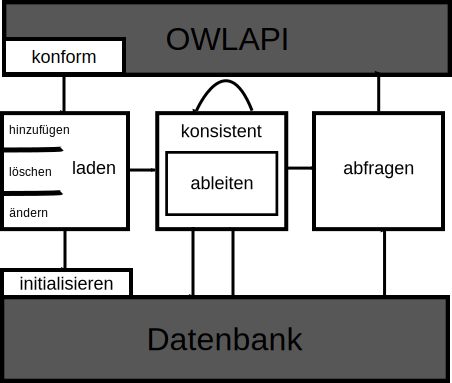
\includegraphics{images/u2r3-workflow.pdf}
	}
\end{center}
\end{figure}

\subsection{Konformität}
Konformität: überprüft, ob die verwendete Syntax im OWL2 RL Profil liegt
laden: bringt die Ontolgoie in das Datenbank-Schema, dabei merkt es an welche Regeln für das ableiten ausgeführt werden sollen
initialisieren: erzeugt das Datenbankschema notfalls, läd Standardwerte und richtet in der Datenbank nötige Funktionen ein
konsistent: ist eine Hülle um dafür zu sorgen, das nur über konsistente Fakten geschlossen wird. Die Häufigkeit kann eingestellt werden.
ableiten:Wendet die Ableitungsregeln an. Die Regelandwendung ist abgschloßen wenn keine neuen Fakten erzeugt werden können.
abfragen: implementiert die Schnittstelle der OWLAPI, mit der man Anfragen an die abgeleiteten Fakten stellen kann

\subsection{OWLAPI Anbindung}

Der obere Teil ist die sogenannte OWLAPI. Die OWLAPI ist eine Bibliothek die das Auslesen von Ontologien in verschiedenen Formaten erlaubt und eine Schlussfolgererschnittstelle für andere Programme zur Verfügung stellt. Durch die Implementierung dieser Schnittstelle in U2R3 ist es für alle Programme zugänglich die mit der OWLAPI arbeiten.
Die Schnittstelle stellt dabei auch eine Liste typischer Abfragen für einen Reasoner dar und kann allein dadurch schon als Messlatte für die Fähigkeiten eines Schlussfolgerers verwendet werden. Das OWLAPI-Projekt ist open-source und in Java implementiert und ist damit auch optimal für die Implementierung von U2R3 geeignet. Neben der reinen Parsertätigkeit kann die OWLAPI auch noch helfen zu überprüfen, ob eine Ontologie im OWL2 RL Profil liegt und nimmt damit weitere Arbeit ab.

\subsection{Das Laden einer Ontologie}

Die Inhalte einer Ontolgie die für das Schlussfolgern wichtig sind, sind die Axiome. Axiome sind dabei Fakten die als allgemein gültig angenommen werden. Sie dienen dazu das Universum der Ontologie zu modellieren und einen Startpunkt für weitere Schlussfolgerungen zu erzeugen.

Alle Axiome werden entsprechend dem MEMA-Prinzip abgelegt. Dabei ist für jedes Axiom genau eine Relation vorgesehen. Falls die Ontologie nicht OWL2 RL konform ist müssen für gewisse Axiome implizite Informationen abgelegt, wie. z.B.

\begin{table}
	\caption{Eine implizite Regel}
	\label{rule-impl}
\begin{center}
	\begin{tabular}{l|l}
    If & then \\ \hline
	T(?i1, ?property, ?i2 ) & T(?property owl:type ObjectProperty) \\
   \end{tabular}
\end{center}
\end{table}


Falls ein Axiom aus komplexen Ausdrücken zusammengesetzt ist werden die Ausdrücke rekursiv abgearbeitet und einzeln behandelt. Zum herstellen der Beziehungen bei komplexen Axiomen werden Platzhalter für die Ausdrücke verwendet. Die Platzhalter die dabei erzeugt werden stammen von der OWLAPI aus der NodeID Klasse und folgen damit dem selben Schema wie auch bei anonymen Individuen.

In folgendem Besipeil soll der komplexe Ausdruck $A \sqcap \exists p.B \sqsubseteq C$ abgespeichert werden. Zur Verdeutlichung wurden Klammern eingebaut.

\begin{equation}
\overbrace{
	(\overbrace{A \sqcap (
		\overbrace{\exists{}p.B}
		^{nid3 \Rightarrow someValuesFrom(nid3, p, B)})}
	^{nid2 \Rightarrow intersectionOf(nid1, nid2), list(nid2, A, nid3)})}
^{nid1 \Rightarrow subClass(nid1, C)} \sqsubseteq C
\end{equation}
Wenn ein Ausdruck nicht direkt abgespeichert werden kann,, dann wird für den Unterausdruck eine \emph{NodeID} erzeugt. Im obigen Beispiel werden drei Stück davon erzeugt. Diese stehen stellvertretend für den Unterausdruck. Es wird dann rekursiv weitergearbeitet bis alle in einfache Ausdrücke aufgelöst werden konnte.

Wenn Fakten in eine Relation geschrieben werden, wird von dieser ein Hinweis (\emph{Reason}) an den Regelprozessor geschickt.

Dieser überprüft die Ursache und legt entsprechende Regeln an, die auf diese Veränderung ausgeführt werden können.

Die abzuarbeitenden Regeln enthalten eine Referenz auf die Fakten, die hinzugekommen sind. Allgemein sind sie so implementiert, das sie nur auf diesen neuen Fakten arbeiten -  auf den sogenannten Deltas - dies ist allerdings nicht in allen Fällen möglich (\emph{cls-int1}), sinnvoll (zu viele verschiedene Kombinationsmöglichkeiten) oder einfach zu komplex und damit fehleranfällig (\emph{prp-spo2}). Falls zwei oder mehrmals eine Regel auf die selben neuen Fakten erzeugt wird bevor sie ausgelöst wird, werden die beiden Regeln zu einer zusammengefasst und können je nach Einstellung neu priorisiert werden.

All diese Regeln sind in einer Warteschleife abgelegt, die beim Laden der Ontologie gefüllt wird und beim Abarbeiten, d.h. dem Realisieren, der Ontologie ausgelesen wird.

Regeln können durch das Erzeugen von neuen Fakten Hinweise für den Regelprozessor geben der daraufhin weitere Regeln anlegt und in die Warteschlange einsortiert.

Der Vorgang des Realisierens ist abgeschlossen, wenn keine Regel neue Fakten und damit neue Regeln erzeugen kann.

Der OWL2 RL Regelsatz garantiert dabei, das es immer zu einem Ende der Regelanwendung kommen wird, egal ob eine gültige oder ungültige Ontologie geladen wird.

Für das Abarbeiten und Erzeugen der Regeln ist hauptsächlich der Regelprozessor verantwortlich. Hier sind noch weitere Einstellungsmöglichkeiten, wie z.B. die parallele Verarbeitung von Regeln vorhanden.


\subsection{Das Schlussfolgern in einer Ontologie}
Das Schlussfolgern in einer Ontologie besteht darus die möglichen Regeln der OWL2 RL SPzeifiaktion anzuwenden. Diese Regeln erzeugen neue Fakten oder überpürfen dieKonsistenz. Der Schlussfolgerer hat seine Arbeit erledigt, wenn keine Regel neue Fakten erzeugen kann, Das sicherzustellen und dabei möglichst wenige Regeln anzuwenden ist seine Aufgabe. Daher wird im folgenden äher beschrieben, wann welche Regeln ausgelöst werden und in welcher Rehenfolge sie angewendet werden.

\subsubsection{Auswertungsstrategien}
Die Auswertungstrategie beschreibt in welcher Reihenfolge der Regelprozessor die Anwendung von Regeln auslöst. 

Der naive Ansatz wäre alle Regeln nacheinander auszuführen, d.h. alles Regeln die implementiert sind anwenden, wenn eine der Regeln dabei neue Fakten erzeugt muss dieser Vorgang wiederholt werden. Dieses Vorgehen ist trotz seiner leichten Umsetzbarkeit nicht implementiert, da der Reasoner damit unnötig viel Arbeit verrichten müssste.

Ein etwas fortgeschrittener Ansatz ist es die Abhängigkeiten der Regeln auszunutzen, d.h. nur wenn für die Prämisse einer Regel überhaupt Fakten vorhanden sind kann diese ausgelöst werden. Das heißt im konkreten, wenn eine Relation die in einer Regel in der Prämisse verwendet wird neue Daten enthält, dann muss diese Regel ausgelöst werden. Dieses Verfahren ist im Schlussfolgerer so umgesetzt.

Es wurde allerdings diese Vorgehen noch etwas weiter verbessert. Veränderungen in verschiedenen Tabellen könnten mehrmals die selbe Regel auslösen, da die Regel mehrere Vorbedingungen  hat. Die Regel wird dann nicht mehrfach ausgelöst sondern es werden erst alle Regeln in eine Warteschlange gesammelt. Wird eine neue Regel ausgelöst wird dann zuerst geschaut, ob diese Regel schon in der Warteschlange vorhanden ist.

Außerdem gibt es hier noch eine Optimierungsmöglichkeit, mit der man noch experimentieren kann. Wenn eine Regel in der Warteschlange erneut eingereiht werden soll, kann man sich entscheiden, ob die Regel an ihrere Stelle in der Schlange verbleibt oder ob sie herausgenommen wird und wieder ans Ende gestellt. Welches der beiden Verfahren besser ist muss sich erst noch in der Praxis zeigen.

In der Konfiguration des u2r3 ist diese Einstellungsmöglichkeit unter dem Namen \emph{EvaluationStrategy} zu finden. Gültige Werte dafür sind \emph{COMMONLAST} oder \emph{RARELAST}

\subsubsection{Regelauslösung}
Für jede Manipulation der Datenbank (DELETE/INSERT) wird eine Reason ausgelöst. Es wird dabei nur eine Reason ausgelöst, egal wieviele Zeilen von der Manipulation betroffen waren. Eine Reason löst dann weitere Actions aus, je nachdem welche Regeln davon betroffen sind.

\begin{verbatim}
DB Manipulation (1) ===> (1) Reason (1) ===> (n) RuleActions
\end{verbatim}


\begin{verbatim}
           Realtion                     Delta
            ######
            ######         <===           #
            ######
                                          |
(welche Regel) |                          | (welche neuen Daten)
               |                          |
                ####>  Reason  <==========

                          | (1)
                          |
                          | (eine Regel mit neuen Daten)
                          |
                          v (n)

                      RuleAction
\end{verbatim}


\subsection{Das Abfragen einer Ontologie}
Das Abfragen in einer Ontologie lässt sich grundlegend in zwei Arten aufteilen. Erstens man hat einen Ausdruck und möchte überpürfen, ob dieser geschlussfolgert worden ist. Diese Art von Abfrage liefert nur ja oder nein zurück. Die zweite Art von Abfrage möchte eine Ergebnismenge zurück. Dabei ist im Gegensatz zur ersten Art von Abfrage eine Variable in der Abfrage, die gefüllt wird.

Bei beiden ist grundsätzlich so, dass das ``Anfrage'' OWL-Konstrukt in eine SQL-ABfrage umgeformt wird. In beiden Fällen kann die Abfrage beantwortet werden egal on die SQL-ABfrage etwas zurückbringt oder nicht. Im zweiten Fall muss aber bei einem Ergebnis daraus noch eine Ergebnis ereugt werden, so das es dem OWLAPI Format entspricht.

\section{Komplexe Ausdrücke}
Was sind komplexe Ausdrücke?
\subsection{Komplexe Ausdrücke finden}
Einfügen von Statements oder Werten nicht gut, weil darüber nicht geschloßen werden kann bzw. wenn darüber Aussagen gemacht werden sollen muss erst geschloßen werden. (zeitaufwendig!)


\section{Aufbau des Schlussfolgerers}


\begin{figure}[htp]
	\caption{Aufbau der Hauptklassen des U2R3 Reasoner}
	\label{schema-aufbau-u2r3}
	
	\tikzstyle{composition}=[->, >=diamond, thick]
	
	\tikzstyle{class}=[rectangle, draw=black, rounded corners, fill=white, drop shadow, text centered, anchor=north, text width=3.5cm, rectangle split, rectangle split parts=1]

	\begin{tikzpicture}[node distance=2cm]
	    \node (U2R3Reasoner) [class]
	        {
	            \textbf{U2R3Reasoner}
	%            \nodepart{second}name
	        };
	        
	    \node (RuleManager) [class, below of= U2R3Reasoner]
	        {
	            \textbf{RuleManager}
	%            \nodepart{second}name
	        };
	        
	     \node (RelationManager) [class, left =0.1cm of RuleManager]
	        {
	            \textbf{RelationManager}
	%            \nodepart{second}name
	        };
	        
	    \node (ReasonProcessor) [class, right =0.1cm of RuleManager]
	        {
	            \textbf{ReasonProcessor}
	            %\nodepart{second}+ classify()
			};

		\draw[composition] (RuleManager.north) -- (U2R3Reasoner.south);
		\draw[composition] (RelationManager.north) -- (U2R3Reasoner.south);
		\draw[composition] (ReasonProcessor.north) -- (U2R3Reasoner.south);

	\end{tikzpicture}
\end{figure}

Das Klassendiagram in Abbildung \ref{schema-aufbau-u2r3} stellt den vereinfachten Aufbau des Schlussfolgerers dar. Die Aufgaben des Reasoner sind dabei in vier Hauptbereich zerlegt.
\begin{enumerate}
  \item Der RelationManger verwaltet die Relationen in der Datenbank und stellt die Verbindung zu dieser her. Darin sind alle Methoden die mit der Erstellung und Veränderung von Tabellenstrukturen zu tun hat enthalten.
  \item Der RuleManager kapselt alle Regeln ab.
  \item Der ReasonProcessor bringt Regeln zur Ausführung. Damit ist er das eigentliche Herz des Schlussfolgerers. Hier wird bestimmt welche Regeln auf welche Relationen angewendet werden und in welcher Reihenfolge.
  \item Der U2R3Reasoner stellt die Schnittstelle nach außen dar. Er nimmt Ontologien, sowie Anfragen an diese Ontologien entgegen.
\end{enumerate}

\section{Auswertungsstrategien}
Modusname: '''!EvaluationStrategy''' := COMMONLAST | RARELAST

== Alle Regeln nacheinander ==
trivial (nicht implementiert, sollte in der !RuleActionQueue umgesetzt werden)

== Abhängigkeiten der Regeln ausnutzen/Regeln in eine Queue packen ==

Regeln zusammenfassen, falls sie mehrmals angefragt werden

 * an ihrer Position in der Queue lassen
 * zurückschieben '''im Moment implementiert''' (siehe !RuleActionQueue)

== Regelauslösung ==
Für jeden Manipulation der Datenbank (DELETE/INSERT) wird/muss eine Reason ausgelöst (werden). Es wird dabei nur eine Reason ausgelöst, egal wieviele Zeilen von der Manipulation betroffen war. Eine Reason löst dann weitere Actions aus, je nachdem welche Regeln davon betroffen sind.


%{{{
DB Manipulation  (1) ===> (1) Reason (1) ===> (n) RuleActions
%}}}

%{{{
           Realtion                     Delta
%            ######
%            ######         <===           #
%            ######
                                          |
(welche Regel) |                          | (welche neuen Daten)
               |                          |
%                ####>  Reason  <==========

                          | (1)
                          |
                          | (eine Regel mit neuen Daten)
                          |
                          v (n)

                      RuleAction

%}}}

\section{Komplexe Ausdrücke}
Was sind komplexe Ausdrücke?
\subsection{Komplexe Ausdrücke finden}
Einfügen von Statements oder Werten nicht gut, weil darüber nicht geschloßen werden kann bzw. wenn darüber Aussagen gemacht werden sollen muss erst geschloßen werden. (zeitaufwendig!)

\begin{verbatim}
    * Was ist der Unterschied zu OWL1 DL/Lite?
    * Was sind Fähigkeiten, die der neue U2R2 haben soll?
          o Schlussfolgern, Konsistenzprüfung, Änderung, Löschung, OWLAPI Anbindung, Konformitätsüberprüfung auf OWL2 RL 
    * Wie konform und semantisch korrekt war U2R2?
    * Was ist der Unterschied in der Menge und Art der Regelimplementierung
          o Welche Techniken wurden verwendet
          o Wieviele wurden implementiert
                + Aussagekraft der Sprachen 
          o Wie komplex sind die implementierten Regeln? Wären alle Regeln aus u2r3 auch in u2r3 implementierbar gewesen, oder wie aufwändig wäre es gewesen diese zu implementieren?
                + Lohnt sich deshalb schon der Umstieg auf ein RDBMS? (einfachere Aufbau, standardisierte Funktionen, größere Funktionsumfang) 
    * Wie wird die Trennung von Klassen und Individuen im MEMA-Modell erhalten?
    
    
        * Welche Fragestellungen gibt es?
    * Wie hängen diese zusammen?
    * Wie können spätere Manipluationen durchgeführt werden?
    * Was ist der Aufwand nach einer Änderung (von Fakten oder Konzepten)?
    * Was ist die Ausdrucksmächtigkeit von OWL2 RL?
    * Was ist die Zeit und Speicher Komplexität von OWL2 RL?
    * Was ist der Unterschied zur Ausdrucksmächtigkeit von U2R2 (1)?
    * Welche Erkenntisse gibt es bereits?
    * Was sind die Fähigkeiten/Ausdrucksmächtigkeiten der verschiedenen Fragmente?
    * Was sind ihre Komplexitäten?
    * Was versteht man unter Truth-Maintenance? 


    * Wie muss dadurch über die entstandenen Daten geschloßen werden?
    * Was sind deduktive Datenbanken?
    * Können die SQL Statements generiert werden?
    * Wie bildet man Regeln allgemein auf SQL ab? RAP?
    * Kann man quadrat. Rekursion im auflösen?
    * Wie sieht das DB-Schema aus?
    * Kann man manche Ableitungsschritte zusammenfassen?
    * Was bringen rekursive Abfragen wirklich? (Es werden dadurch ja auch andere Regeln angestoßen und dann müssen die rekursiven wieder ran)
    * Wie wandelt man die Ontologie in INSERTs um? 
\end{verbatim}


\section{Zurückziehen von Fakten}
Das Einfügen von Fakten, die man löschen will um herauszufinden, welche gleich sind, um sie danach wieder zu löschen macht keinen großen Sinn. Erstens ist es Recht aufwendig zu implementieren. Zweitens müsste nach dem Einfügen neuer Fakten ersteinmal wieder die Ableitungsregeln ausgeführt werden. Das zerstört den Vorteil den man sich durch forward-chaining mit direct-materialisation erkauft hat sofort wieder und bringt außerdem auch Nachteille mit sich wenn man noch nicht komplett fertig war mit dem Schlussfolgern.
Daher muss es ein Verfahren geben die zu löschenden Fakten zu finden ohne sie vorher einfügen zu müssen.

\section{Finden von Fakten}


%Kapitel Realisierung
\chapter{Realisierung}

\section{Regelumsetzung allgemein}
\label{abschnitt-regelumsetzung}
Regeln sind hier sogenannte Inferenzprozeduren, das sind automatisierte Verfahren zur Berechnung logischer Folgerungen. Inferenzprozeduren sind bereits aus der Aussagenlogik bekannt.

\begin{table}[htb]
\begin{center}
	\begin{tabular}{l}
	A$\rightarrow$B \\
	A \\
	\hline
	B
	\end{tabular}
\end{center}
	\caption{Modus ponens}
	\label{table-modus-ponens}
\end{table}

\begin{table}[htb]
\begin{center}
	\begin{tabular}{l}
	A$\rightarrow$B \\
	$\neg$B \\
	\hline
	$\neg$A
	\end{tabular}
\end{center}
	\caption{Modus tollens}
	\label{table-modus-tollens}
\end{table}

Diese beiden Ableitungsregeln [\ref{table-modus-ponens}, \ref{table-modus-tollens}] erlauben es, die beiden Aussagen in der Prämisse durch die Schlussfolgerung zu ersetzen. Für einen Schlussfolgerer mit direct-materialization werden, die Prämissen nicht ersetzt sondern weiterhin erhalten. Es könnte ja möglich sein das weitere Ableitungsschritte damit möglich sind oder das spätere Anfragen auf diese Aussagen abzielen. Mit einer Ableitungsregel kann also die Aussagenbasis vergrößert werden.

Es sind dabei jedoch nicht alle Ableitungsregeln gültig.
\begin{table}[htb]
\begin{center}
	\begin{tabular}{l}
	A$\rightarrow$B \\
	B \\
	\hline
	A
	\end{tabular}
\end{center}
	\caption{ungültige Ableitung}
	\label{table-invalid-inferred}
\end{table}
Abbildung \ref{table-invalid-inferred} ist z.B. kein gültiger Schluss.

Eine Menge von vernünftigen Ableitungsregeln zu finden ist keine leichte Aufgabe. Dabei eine möglichst große Ausdrucksmächtigkeit zu erhalten, ohne die Komplexität der Regeln aus den Augen zu verlieren wurde versucht mit dem OWL2 RL Fragement zu erreichen.

\subsection{Regelbeispiele}
\label{abschnitt-regelbeispiele}
In diesem Teil der Regelumsetzung wird an konkreten Beispielen gezeigt, wie eine Umsetzung der OWL2 RL Regeln in SQL möglich ist. Die SQL Abfragen benutzen dabei die vorher im MEMA-Prinzip erstellen Relationen

Die Abfragen werden zunächst allgemein an einfachen Regeln prinzipiell erklärt, danach wird auf die Sonderfälle eingegangen.

Insgesamt kann dabei in fünf Kategorien unterschieden werden:
\begin{itemize}
  \item Gewöhnliche Regeln: Dabei werden verschiedene Fakten miteinander verknüpft, so dass dabei neue Fakten entstehen können. Diese Regeln sind alle sehr schematisch umsetzbar.
  \item Listenregeln: Hier werden Listen von Fakten bearbeitet. Dabei ist nicht klar wie viele Elemente eine Liste enthält. Dies kann zu einem Problem werden, wenn man die Entstehungsgeschichte von Fakten, z.B. für das Löschen mitabspeichern will. Hier muss man gesondert darauf achten, dass diese Information der Entstehung nicht verloren geht.
  \item Inkonsistenzregeln: Sie sind ähnlich der gewöhnlichen Regeln, erzeugen allerdings keine neuen Fakten. Falls sie neue Fakten erzeugen könnten, bedeutet dies eine Inkonsistenz in der Ontologie.
  \item Regeln für Datentypen: Für typisierte Literale werden einige Überprüfung bzgl. der Gleichheit untereinander und der Konformität zu den in OWL2 RL eingebauten Datentypen durchgeführt.
  \item Einmalige Regeln: Einige Regeln haben keine Vorbedigung. Diese werden einmal zum Start des Regelprozessors ausgeführt.
\end{itemize}

\subsubsection{Einmalige Regeln}

\begin{table}[htb]
\begin{center}
	\begin{tabular}{l|l}
	if & then \\ \hline
	true & T(owl:Thing, rdf:type, owl:Class)
	\end{tabular}
\end{center}
	\caption{Die Regel cls-thing}
	\label{rule-cls-thing}
\end{table}


Diese Regel \ref{rule-cls-thing} wird einmal zu Beginn in die Liste der Regelanwendungen gesteckt. Sie sorgt dafür das dieses Faktum eingefügt wird.

In SQL lautet dies:
\begin{lstlisting}[language=SQL]
INSERT INTO classAssertionEnt (entity, class)
	VALUES ('owl:Thing', 'owl:Class')
\end{lstlisting}

\subsubsection{Inkonsistenzregeln}
Inkonsistenzregeln erzeugen keine Fakten. Sie versuchen aber gewisse Fakten zu finden, die im Widerspruch zu einander stehen.

\begin{table}[htb]
\begin{center}
	\begin{tabular}{l|l}
	if & then \\ \hline
	T(?x, rdf:type, owl:Nothing) & false
	\end{tabular}
\end{center}
	\caption{Die Inkonsistenzregel cls-nothing2}
	\label{rule-cls-nothing2}
\end{table}


Dies wird in folgende SQL-Abfrage umgewandelt:
\begin{lstlisting}[language=SQL]
SELECT 1
FROM classAssertionEnt
WHERE class = 'owl:Nothing'
\end{lstlisting}

Die Relation classAssertionEnt ist die Relation, die die type-Beziehung speichert. Ist darin eine Zeile zu finden, die als type die KLasse owl:Nothing hat wird eine Zeile zurückgegeben. Falls also diese Abfrage eine oder mehrere Zeilen erzeugt liegt eine Inkonsistenz vor.

\subsubsection{Gewöhnliche Regeln}
Gewöhnliche Regeln erzeugen neue Fakten in der Datenbank. Eine einfache Regel ist hier eq-sym:

\begin{table}[htb]
\begin{center}
	\begin{tabular}{l|l}
	if & then \\ \hline
	T(?x, owl:sameAS, ?y) & T(?y, owl:sameAS, ?x)
	\end{tabular}
\end{center}
	\caption{Die gewöhnliche Regel eq-sym}
	\label{rule-eq-sym}
\end{table}

Dies wird wie folgt in SQL überführt:
\begin{lstlisting}[language=SQL]
INSERT INTO sameAs (left, right)
SELECT right, left
FROM sameAs
\end{lstlisting}

Wie die Abfrage zu Stande kommt sollte klar sein. Allerdings wurden in dieser Umwandlung schon einge Dinge vereinfacht, die in der Implementierung so nicht gemacht wurden.

\begin{enumerate}
  \item Was passiert wenn eine Zeile eingefügt werden soll, die schon enthalten ist?
  \item Wie würde man hier die Delta-Iteration einsetzen können, um nicht immer auf alle Fakten schließen zu müssen?
  \item Wie kann man die Entstehungsgeschiechte von neuen Fakten mitschreiben, um später effizientes Löschen zu ermöglichen.
\end{enumerate}

Diese Punkte werden jeweils in ihren speziellen Abschnitten behandelt. Um die Beispiele nicht unnötig komplizierter zu machen wird hier nicht näher darauf eingegangen.

Ein komplexeres Beispiel ist die Verknüpfung von Fakten, um auf neue Fakten schließen zu können, z.B. in der Regel eq-rep-s:
\begin{table}[htb]
\begin{center}
	\begin{tabular}{m{4.5cm}|m{4cm}}
	if & then \\ \hline
	T(?s1, owl:sameAs, ?s2),\newline T(?s1, ?p, ?o) & T(?s2, ?p, ?o)
	\end{tabular}
\end{center}
	\caption{Die Regel eq-rep-s}
	\label{rule-eq-rep-s}
\end{table}

Die Verknüpfung wird durch einen JOIN auf die entsprechende Spalte realisiert.

\begin{lstlisting}[language=SQL]
INSERT INTO objectPropertyAssertion(subject, object, property)
SELECT sa.right, opa.property, opa.object
FROM objectPropertyAssertion AS opa
INNER JOIN sameAs AS sa
	ON sa.left = opa.subject
\end{lstlisting}

\subsubsection{Listenegeln}
Dabei können Listenregeln auch Regeln sein die neue Fakten erzeugen oder Inkonsistenzen überprüfen. Eine Inkonsistenzregel mit einer Liste ist z.B. prp-adp:
\begin{table}[htb]
\begin{center}
	\begin{tabular}{M{7cm}|M{1.2cm}|M{2.5cm}}
	if & then & \\ \hline
	T(?x, rdf:type, owl:AllDisjointProperties),\newline
	T(?x, owl:members, ?y),\newline
	LIST[?y, ?$p_1$, \ldots, ?$p_n$],\newline
	T(?u, ?$p_i$, ?v),\newline
	T(?u, ?$p_j$, ?v) & false & für alle $1 \leq i < j \leq n$
	\end{tabular}
\end{center}
	\caption{Die Listenregel prp-adp}
	\label{rule-prp-adp}
\end{table}


Bei der Erstellung der Abfrage kann man rein schematisch vorgehen. Es werden alle Relation auf den Variablen mit den gleichen Namen gejoint. Liefert dese Abfrage ein Ergebnis zurück ist eine Inkonsistenz vorhanden.

\begin{lstlisting}[language=SQL]
SELECT 1
FROM classAssertionEnt AS ca
INNER JOIN members AS m ON ca.entity = m.class
INNER JOIN list AS l ON m.list = l.name
INNER JOIN objectPropertyAssertion AS opa1
	ON opa1.property = l.property
INNER JOIN objectPropertyAssertion AS opa2
	ON opa2.property = l.property
WHERE opa1.subject = opa2.subject AND opa1.object = opa2.object
	AND ca.class = 'owl:AllDisjointProperties'
\end{lstlisting}

Tatsächlich wird hier mehr gemacht als nötig ist. Die \emph{subject} und \emph{object} Spalten werden von beiden Seiten miteinander verglichen. Es wäre aber nur eine nötig. So ist es allerdings einfacher und natürlicher in SQL Syntax zu implementieren.

Im Falle der Regel eq-diff2 muss eine Tabelle doppelt importiert werden, um wirkliche alle Fakten mit einander vergleichen zu können. Die ursprüngliche Regel.
\begin{table}[htb]
\begin{center}
	\begin{tabular}{M{7cm}|M{1.2cm}|M{2.5cm}}
	if & then & \\ \hline
	T(?x, rdf:type, owl:AllDifferent),\newline
	T(?x, owl:members, ?y),\newline
	LIST[?y, ?$z_1$, \ldots, ?$z_n$],\newline
	T(?$z_i$, owl:sameAs, ?$z_j$) & false & für alle $1 \leq i < j \leq n$
	\end{tabular}
\end{center}
	\caption{Die Listenregel eq-diff2}
	\label{rule-eq-diff2}
\end{table}


Würde man hier streng nach Schema vorgehen würde die sameAs Relation nur einmal in der Abfrage auftauchen. Das würde allerdings nicht alle Kombinationen erzeugen. Die Abfrage ist damit sehr ähnlich der obigen und wird hier ausgespart.

Ein besonderer Typ der Listenregel ist z.B. cls-oo, diese Regel erzeugt mehrere Fakten. Das ist aber in der Umsetzung kein Problem.
\begin{table}[htb]
\begin{center}
	\begin{tabular}{m{4.5cm}|m{4cm}}
	if & then \\ \hline
 	T(?c, owl:oneOf, ?x),\newline
 	LIST[?x, ?$y_1$, \ldots, ?$y_n$]
								 	&
								 	T(?$y_1$, rdf:type, ?c),\newline
								 	\ldots,\newline
								 	T(?$y_n$, rdf:type, ?c)
	\end{tabular}
\end{center}
	\caption{Die Listenregel cls-oo}
	\label{rule-cls-oo}
\end{table}


\subsubsection{Datentypenregeln}
Die Regeln zur Überprüfung der Datentypen ist nicht komplizierter, allerdings eine effiziente Umsetzung ist hier das Problem. Hier ist vor allem die dt-eq Regel das Problem.
\begin{table}[htb]
\begin{center}
	\begin{tabular}{l|l|M{3cm}}
	if & then & \\ \hline
	true & T(lt1, owl:sameAs, lt2) & für alle Literale lt1 und lt2 mit dem selben Datenwert
	\end{tabular}
\end{center}
	\caption{Die Datentyperegel dt-eq}
	\label{rule-dt-eq}
\end{table}


Die aktuelle Umsetzung versucht sich möglichst nah an das MEMA-Prinzip und die Regel zu halten. Optimierungen sind hier noch wesentlich vorhanden.

\begin{lstlisting}[language=SQL]
INSERT INTO sameAsLit (left, right)
SELECT ca1.literal, ca2.literal
FROM classAssertionLit AS ca1
CROSS JOIN classAssertionLit AS ca2
WHERE isSameLiteral(ca1.literal, ca2.literal)
\end{lstlisting}

Zum einen wird hier ein CROSS JOIN verwendet der eine der aufwendigsten Datenbankoperationen ist, außerdem können Literale nicht mit den üblichen Datenbankoperatoren verglichen werden. Hierzu wurde eine eigene Datenbankmethode geschrieben die dies übernimmt. Die Datenbankmethode ruft eine Java-Routine auf, die dann den eigentlichen Vergleich vornimmt. Diese beiden Verlangsamungen sind noch nicht genug. In der aktuellen IMplementierung sind nicht gleich alle Literal in der Relation, sondern können später noch hinzukommen, d.h. das diese Regel öfters aufgerufen werden kann. Hier ist also noch Potential für eine Optimierung vorhanden.


\subsubsection{Spezialfälle} 
In die Kategorie der Spezialfälle fallen drei Regeln aus OWL2 RL. Sie haben im Gegensatz zu den anderen Regeln eine variable Anzahl von Fakten in der Prämisse. Diese Fakten sind allerdings nur indirekt über eine Liste verknüpft.

Die erste Regel ist prp-spo2, sie erweitert eine Liste in eine Kette von Eigenschaften.
\begin{table}[htb]
\begin{center}
	\begin{tabular}{m{7cm}|m{3cm}}
	if & then \\ \hline
	T(?p, owl:propertyChainAxiom, ?x),\newline
	LIST[?x, ?$p_1$, \ldots, ?$p_n$],\newline
	T(?$u_1$, ?$p_1$, ?$u_2$),\newline
	T(?$u_2$, ?$p_2$ ?$u_3$),\newline
	\ldots,\newline
	T(?$u_n$, ?$p_n$, ?$u_{n+1}$) & T(?$u_1$, ?p, ?$u_{n+1}$)
	\end{tabular}
\end{center}
	\caption{Der Spezialfall prp-spo2}
	\label{rule-prp-spo2}
\end{table}

Die Kette muss dabei einen Start und ein Ende haben und die Glieder der Kette müssen untereinander verbunden sein. Die Variable ?u2 wird einmal als object und einmal als subject verwendet. Wenn das so ist ergeben der Start, die Eigenschaft und das Ende einen neues Faktum.

Diese Regel ist in SQL in zwei Schritten übersetzt worden. Zunächst eine Hilfsabfrage die in der späteren Abfrage mehrmals verwendet wird.

\begin{lstlisting}[language=SQL]
SELECT vopa.subject as vorgaenger,
       opa.subject  AS start,
       opa.object   AS ende,
       nopa.object  as nachfolger,
       l.name       AS lname,
       anzl.anz
FROM   list AS l
       INNER JOIN objectpropertyassertion AS opa
         ON opa.property = l.element
       INNER JOIN (SELECT   name,
                            COUNT(name) AS anz
                   FROM     list
                   GROUP BY name) AS anzl
         ON anzl.name = l.name
       LEFT OUTER JOIN objectpropertyassertion AS vopa
         ON vopa.object = opa.subject
       LEFT OUTER JOIN objectpropertyassertion AS nopa
         ON nopa.subject = opa.object
\end{lstlisting}

Diese Abfrage erzeugt ein Ergebnis in der alle objectPropertyAssertions einer Liste mit ihrem Vorgänger und Nachfolger aufgelistet sind. Außerdem wird die Anzahl der Elemente in der Liste mitgeführt.

\begin{lstlisting}[language=SQL]
INSERT INTO objectPropertyAssertion
           (subject,
            property,
            object)
SELECT start.start,
       pc.property,
       ende.ende
FROM   (SELECT   lname,
                 anz
        FROM     (--- Unterabfrage fuer gueltige Liste ---)
        GROUP BY lname
        HAVING   COUNT(lname) = anz) AS thel
       INNER JOIN (SELECT lname,
                          start
                   FROM   (--- Unterabfrage fuer Vorgaenger ---)
                   WHERE  vorgaenger IS NULL) AS start
         ON start.lname = thel.lname
       INNER JOIN (SELECT lname,
                          ende
                   FROM   (--- Unterabfrage fuer Nachfolger ---)
                   WHERE  nachfolger IS NULL) AS ende
         ON ende.lname = thel.lname
       INNER JOIN propertyChain AS pc
         ON pc.list = thel.lname
\end{lstlisting}

Die vorher beschriebene Abfrage wird mehrmals eingesetzt. Sie erzeugt einerseits nur gültige Liste. Das ist die erste Abfrage. Die zweite Unterabfrage wählt das Startelement aus und die dritte das Endeelement. Am Ende wird es noch auf die eigentliche propertyChain gejoined.

Die zweite Regel überprüft, ob ein Invidivum in allen Teilen einer Schnittmenge vorhanden ist. Falls ja wird es der Klasse dieser Schnittmenge hinzugefügt.
\begin{table}[htb]
\begin{center}
	\begin{tabular}{m{5cm}|m{3.5cm}}
	if & then \\ \hline
	T(?c, owl:intersectionOf, ?x),\newline
	LIST[?x, ?$c_1$, ..., ?$c_n$],\newline
	T(?y, rdf:type, ?$c_1$),\newline
	T(?y, rdf:type, ?$c_2$),\newline
	\ldots,\newline
	T(?y, rdf:type, ?$c_n$) & T(?y, rdf:type, ?c) 	 
	\end{tabular}
\end{center}
	\caption{Der Spezialfall cls-int2}
	\label{rule-cls-int2}
\end{table}


\begin{lstlisting}[language=SQL]
INSERT INTO classAssertionEnt
           (entity,
            class)
SELECT   clsA.entity AS entity,
         int.class   AS class
FROM     (SELECT   name,
                   COUNT(name) AS anzahl
          FROM     list
          GROUP BY name) AS anzl
         INNER JOIN list AS l
           ON anzl.name = l.name
         INNER JOIN classAssertionEnt AS clsA
           ON l.element = clsA.class
         INNER JOIN intersectionOf AS int
           ON int.list = l.name
GROUP BY l.name,
         clsA.entity,
         int.class
HAVING   COUNT(l.name) = anzl.anzahl
\end{lstlisting}

Diese Abfrage wurde auch wesentlich vereinfacht. Für die Abspeicherung einer Historie dürfen die Fakten erst danach gruppiert werden, dann wäre allerdings keine Überprüfung mit HAVING möglich.

Die aktuelle Umsetzung kann im Wiki oder im Code gefunden werden.

Die dritte Abfrage prp-key überprüft ob zwei Individuen das Gleiche sind. Dies geschieht an Hand einer Liste  von Key-Eigenschaften, wenn diese übereinstimmen sind auch die die Individuen gleich.
\begin{table}[htb]
\begin{center}
	\begin{tabular}{m{4.5cm}|m{4cm}}
	If & then \\ \hline
	T(?c, owl:hasKey, ?u),\newline
	LIST[?u, ?$p_1$, \ldots, ?$p_n$],\newline
	T(?x, rdf:type, ?c),\newline
	T(?x, ?$p_1$, ?$z_1$),\newline
	\ldots,\newline
	T(?x, ?$p_n$, ?$z_n$),\newline
	T(?y, rdf:type, ?c),\newline
	T(?y, ?$p_1$, ?$z_1$),\newline
	\ldots,\newline
	T(?y, ?$p_n$, ?$z_n$) & T(?x, owl:sameAs, ?y)
	\end{tabular}
\end{center}
	\caption{Der Spezialfall prp-key}
	\label{rule-prp-key}
\end{table}


Die Abfrage ist der Einfachheit ebenfalls in zwei Teile zerlegt. Die Unterabfrage, die mehrmals verwendet wird, erzeugt zunächst eine gültige Liste von Individuen die über eine Eigenschaft mit dem gleichen Objekt verbunden sind.
\begin{lstlisting}[language=SQL]
SELECT pax.subject, sl.name, anzl.anz
FROM list AS sl
        INNER JOIN (
                SELECT name, COUNT(name) AS anz
                FROM list
                GROUP BY name
        ) AS anzl
                ON anzl.name = sl.name
        INNER JOIN (
                SELECT id, subject, property, object
                FROM objectPropertyAssertion
                UNION
                SELECT id, subject, property, object
                FROM dataPropertyAssertion
        ) AS pax
                ON sl.element = pax.property
        INNER JOIN (
                SELECT id, subject, property, object
                FROM objectPropertyAssertion
                UNION
                SELECT id, subject, property, object
                FROM dataPropertyAssertion
        ) AS pay
                ON sl.element = pay.property
                AND pax.property = pay.property
                AND pax.object = pay.object
GROUP BY pax.subject, sl.name
--- Es werden alle Listenelemente doppelt erzeugt
HAVING COUNT(sl.name) = 2*anz
\end{lstlisting}

Diese Liste wird dann in der folgenden Abfrage zweimal verwendet um zwei Individuen miteinander verleichen zu können.
\begin{lstlisting}[language=SQL]
INSERT INTO sameAsEnt (left, right)
SELECT ca1.entity AS left, ca2.entity AS right
FROM hasKey AS hk
     INNER JOIN list AS l
             ON l.name = hk.list
     INNER JOIN classAssertionEnt AS ca1
            ON ca1.class = hk.class
     INNER JOIN classAssertionEnt AS ca2
            ON ca2.class = hk.class
     INNER JOIN (--- ...Unterabfrage... ---) AS valid1
                ON valid1.subject = ca1.entity
     INNER JOIN (--- ...Unterabfrage... ---) AS valid2
                ON valid2.subject = ca2.entity
\end{lstlisting}

\section{Delta-Iteration}
\label{abschnitt-delta-iteration}

Unabhängig von der Art der delta-Iteration muss immer der Ausführungskontext bekannt sein, d.h. welche delta-Iteration ist aktiv, auf welches delta wird gearbeitet. Ein delta muss dabei die Information enthalten auf welcher Relation es arbeitet und auf welchen Teil. Zum Ausführungskontext gehört je nach Modus auch noch die Information, ob eine Regel schon auf das Ziel delta angewendet wurde.

Die delta-Iteration ist ein Verfahren, um bei Regelanwendungen, die Datenmenge so zu reduzieren, das nur solche enthalten sind, die noch nicht berücksichtigt wurden und somit die tatsächlich zu betrachtenden Menge zu reduzieren.

Während der ersten Entwicklung sind dabei zwei Varianten der delta-Iteration klar geworden. Diese tragen im folgenden die Namen \emph{immediate} delta-Iteration und \emph{collective} delta-Iteration. Timo Weithöhner hat in seiner Implementierung die collective delta-Iteration verwendet.

\subsection{Immediate delta-Iteration}

Hierbei erzeugt jede Regelanwendung sofort ihr eigenes Delta, mit dem weitergearbeitet werden kann. Wenn Zeilen erzeugt wurden, wird sofort das dazugehörige Delta erzeugt und dafür alle notwendigen Regelanwendungen ausgelöst.

Im folgenden ist ein Beispiel gegeben, wie der Ablauf bei der Anwendung einer Regel ist die neue Fakten erzeugt hat und wie diese dann verarbeitet wird. Angenommen die Regel \emph{eq-ref-s} erzeugt neue Fakten, diese landen in einem Delta der \emph{sameAs}-Relation. Das löst eine ``Reason'' aus mit der Information welches Delta neue Fakten enthalten hat. Wenn der Regelprozessor diese erhält erzeugt er für diese Kombination sog. RuleActions, d.h. er bringt alle Regeln die auf diesem delta arbeiten in eine Warteschlange. Zu jeder Regel speichert er den Ausführungskontext, auf den sie angewendet werden soll mit ab. Die Regelanwendungen warten dann bis sie zur Ausführung gebracht werden.

\begin{verbatim}
Regel: eq-ref-s //neue Fakten
=> delta sameas
   => new Reason(sameas, delta)
      => new RuleAction(eq-sym, delta)
         new RuleAction(eq-trans, delta)
         new RuleAction(eq-rep-s, delta)
         new RuleAction(eq-rep-p, delta)
         new RuleAction(eq-rep-o, delta)
         new RuleAction(eq-diff1, delta)
         new RuleAction(eq-diff2, delta)
         new RuleAction(eq-diff3, delta)
\end{verbatim}

Der Regelprozessor ist dann auch verantwortlich die Ausführung der Regelanwendungen zu starten. Das passiert in einer Schleife, die die Elemente der Warteschlange abarbeitet bis keine weiteren Elemente vorhanden sind.

Dies ist im folgenden Code \ref{code-immediate-delta-iteration} schematisch dargestellt:

\begin{figure}[htp]
	\caption{Abarbeitung der RuleActions im immediate Modus.}
	\label{code-immediate-delta-iteration}
	\begin{lstlisting}[language=Java]
while(action = rulesToApply.popAction()) {
	action.rule.apply(action.delta);
	
	if (!(rulesToApply.contains(delta)) {
		delta.addToRelation();
		delta.drop();
		delta == null;
	}
}
	\end{lstlisting}
\end{figure}


Der Vorteil dieser Vorgehensweise ist das es besser parallelisiert werden kann, da so viele Regelanwendungen wie möglich gleichzeitig angewandt werden können. Die Parallelisierung ist eines der Ziele die eventuell in der Zukunft umgesetzt werden sollen.

Der Nachteil ist das viele Deltas gleichzeitig entstehen und insgesamt mehr Regel angewendet werden müssen. Die Deltas enthalten unter Umständen nur wenig Inhalt, d.h. die Abfragen arbeiten auf kleineren Datenmenge aber ein Datenbanksystem lohnt sich eventuell erst wirklich bei großen Datenmengen. Es muss nicht zwangsläufig schlecht sein, aber es ist nicht unbedingt klar wie sich das auf ein DBMS auswirkt.

\subsection{Collective delta-Iteration}

Vom aktuellen Stand einer Relation werden erst einmal alle Änderungen in einer Hilfsrelation gesammelt. Sind alle abgearbeitet, wird das Delta erstellt und die nächste Phase beginnt.

\begin{verbatim}
Regel: sameas-eq-ref-s //neue Fakten
=> aux sameas
\end{verbatim}

\begin{figure}[htp]
	\caption{Abarbeitung der RuleActions im immediate Modus.}
	\label{code-immediate-delta-iteration}
	\begin{lstlisting}[language=Java]
do {
	while (action = list.popAction()) {
		action.rule.apply(action.delta);
	}
}
while (applyRelations()); //WAIT --- SYNC

boolean applyRelations() {
	for(r : relations)
		r.applyAux();
		return relations.wereDirty()
}

applyAux() {
	createDelta;
	addDelta();
	clearAux();
	new Reason(relation, delta);
}
	\end{lstlisting}
\end{figure}

Vorteile:
\begin{itemize}
  \item Es gibt immer nur eine Hilfsrelation und ein Delta, also eine fixe Anzahl an Tabellen.
  \item Es werden evtl. größere Menge an neuen Fakten zusammengefasst. Das muss nicht notwendiger weise gut sein.
\end{itemize}

Ein Nachteil ist, das die Parallelisierung nicht vollständig durchgeführt werden kann, da zu gewissen Zeitpunkten (Zeile 6), die Regelanwendung unterbrochen wird und die Ausführung wieder synchronisiert werden muss.

\subsection{Simulation}

Die collective delta-Iteration kann mit Hilfe der immediate delta-Iteration und ein paar Änderungen umgesetzt werden. Dazu dürfen die Relationen nicht sofort neue Hinweise an den Regelprozessor schicken, sondern es gibt eine eigene Phase nach dem Abarbeiten aller Regeln. Dabei wird erst der Inhalt der Deltas in die Haupttabelle übernommen und es werden die Hinweise an den Regelprozessor geschickt.

Die Hilfstabelle in der die Daten für die Runde zwischengespeichert werden ist das Delta, das neu angelegt wird. Die alte Hilfstabelle wird zum Delta der aktuellen Runde.

Die Implementierung des u2r3 unterstützt beide Varianten der delta-Iteration. Diese können in der Konfigurationsdatei mit der Option DeltaIteration verändert werden. Gültige Werte sind \emph{COLLECTIVE} oder \emph{IMMEDIATE}.



\section{sonstige Punkte: Herausforderungen und Lösungen}
\section{Löschung (\& Änderung)}

Wie aus dem Grundlagen Kapitel \ref{kapitel-grundlagen} bekannt ist handelt es sich bei OWL2 RL um eine monotone Logik. Damit ist das Hinzufügen von Fakten kein Problem, da es sich nicht auf schon geschlussfolgerte Fakten auswirkt. In der Implementierung ist damit die Änderung von Fakten damit umgesetzt, das die zu ändernden Fakten gelöscht und dann die neuen Fakten wieder hinzugefügt werden. Die Änderung von Fakten ist damit auf die Löschung von Fakten reduzierbar.

Allgemein gibt es zwei Arten wie die Löschung von Fakten umgesetzt werden kann. Der naive Ansatz wär es, wenn ein Faktum gelöscht werden soll, werden alle bisher geschlussfolgerten Ergebnisse verworfen und der Schlussfolgerungsprozess wird danach von vorne gestartet. Ein optimierter Ansatz wäre es, das ein Faktum das gelöscht wird nur die Löschung von daraus geschlussfolgerten Ergebnissen auslöst. Dieses Vorgehen wurde im Schlussfolgerer umgesetzt und im folgeden näher beschrieben. Zunächst die grundlegenden Bedingungen für das Löschen von Fakten:

\begin{itemize}
  \item Fakten die hergeleitet wurden können nicht gelöscht werden.
  \item Fakten die keine Ableitungen verursacht haben können gelöscht werden.
  \item Fakten die eine Ableitung verursacht haben können nur gelöscht werden, wenn alle ihre Ableitungen gelöscht werden.
\end{itemize}

Um zu ermöglichen, dass das Löschen eines Faktums nur Ergebnisse entfernt die daraus abgeleitet wurden wird die Ableitungsreihenfolge abspeichern mit abgespeichert. Durch diesen zusätzlichen Aufwand soll die Manipulation an der Ontologie beschleunigt werden.

Dabei ist die Frage wichtig, woher etwas abgeleitet ist. Regeln erzeugen diese Fakten, aber damit eine Regel ausgelöst wird sind eigentlich die Fakten verantwortlich. Das Problem hierbei ist, das unterschiedliche Regeln eine unterschiedliche Anzahl an Fakten in der Prämisse verwenden. Die drei Spezialregeln sind dabei besonders schlimm da sie eine theoretisch beliebig große Anzahl Fakten in der Prämisse verwendet.

Gut ist hingegen das durch das MEMA Prinzip die Unterscheidung zwischen T-Box und A-Box aufgehoben wird. Der Regelsatz von OWL2 RL nimmt darauf auch keinen besonderen Bezug. Damit ist möglich für Löschungen in der T-Box und in der A-Box das selbe Verfahren verwenden zu können.

\subsection{Abspeichern der Ableitungsreihenfolge}
Die ApplicationRules sind die Klasse aller Regeln die neue Fakten erzeugen können. Diese wurden so erweitern, dass sie von jeder verwendeten Tabelle in der Regel, die id der Zeile mitliefert. Jede Tabelle wurde so ausgestatte das jede Zeile als jeder Fakt eine eindeutige Nummer hat. So kann jedes Konstrukt einer Tabelle über eine Nummer angesprochen werden, egal wieviele Unterelemente dieses Konstrukt hat. Das entspricht sehr dem MEMA-Schema, da durch eine id eine klare, einheitlich Historien-Tabelle angelegt werden kann, die unabhängig von unterschiedlichen Axiom-Konstrukten ist. Die ids müssen einzigartig pro Tabelle sein.

Die Anzahl der Spalten die eine Regelanwendung für die Angabe der Historiendaten ist von Regel zu Regel unterschiedlich aber dabei immer für jede Regel fest. Davon ausgenommen sind die drei Spezialregeln. Wie die Historiendaten hier mitgeschrieben werden, wird in Abschnitt \ref{abschnitt-aufblaehung} geklärt.

Danach müssen die Historiendaten in eine seperate Referenztabelle (history \ref{relations-list-history}). Hier wird zu einer id und einer Tabelle, die Quelldaten woher dieser Fakt stammt ebenfalls in Form von einer id und Tabelle abgepseichert.

Im nachfolgendes Beispiel wird die Situation angenommen das eine Subklassenbeziehung zwischen A,B, und B,C besteht. Damit besteht auch eine Subklassenbeziehung zwischen A,C. All diese Ausdrücke sind mit einer eindeutigen id identifizierbar.
\begin{verbatim}
subClass(A,C) := subClass(A,B), subClass(B,C)
   id_neu             id_x           id_y
\end{verbatim}

Dadurch werden folgende Zeilen in der Historietabelle angelegt.

\begin{table}[htb]
\begin{center}
\begin{tabular}{l|l}
ID & QuellID \\ \hline
$id_{neu}$ & $id_x$ \\
$id_{neu}$ & $id_y$
\end{tabular}
\end{center}
\caption{Anlegen einer Ableitungshistorie}
\label{table-inference-history}
\end{table}
Um in deltas schon eine deterministische id vergeben zu können wird eine tabellenübergreifende Sequence verwendet. Das ist eine Möglichkeit in einer Datenbank Standardwerte für Spalten aus einer zentralen Stelle vergeben zu können.

\subsection{Löschablauf}
Man beginnt das Löschen eines Axioms damit das man seine id bestimmt. Dann überprüft man, ob die id in der Historientabelle vorhanden ist. Wenn ja, dann alle Abhängigkeiten finden und rekursiv diese löschen. Danach den Wert selbst löschen. 

z.B.: $subClass(B,C) \Rightarrow id_y$
\begin{lstlisting}[language=SQL]
SELECT id FROM Historie WHERE quelle = $id_y$

while(id)
	delete(id)
	DELETE FROM Historie WHERE id = id

DELETE FROM subClass WHERE id = $id_y$
\end{lstlisting}


Nachdem Fakten gelöscht wurde müssen ebenfalls Regeln ausgelöst werden, da es sein könnte das gelöschte geschlussfolgerte Ergebnisse auch über andere Fakten ableitbar gewesen wären. 
Hier wär auch ein naiver Ansatz möglich, indem man alle Regeln auf alle bekannt Fakten anwendet. Es wurde aber ein effizienteres Verfahren implementiert, so dass nur Regeln ausgelöst werden, die Fakten in den Relationen erzeugen können aus denen etwas gelöscht wurde.
Um entscheiden zu können welche Regeln ausgelöst werden sollen, müssen die Relationen wissen welche Regeln in ihnen neue Fakten erzeugen können. Diese Regeln müssen dann ausgelöst werden im Gegenteil zu ''normalen'' Inferenzregeln.

Für die Unterscheidung wurden zwei verschiedene Reason eingeführt werden.
\begin{itemize}
  \item AdditionReason (wenn der Grund durch das Hinzufügen eines Faktes entstanden ist)
  \item DeletionReason (wenn der Grund durch das Löschen eines Faktes entstanden ist)
\end{itemize}

Der Modus mit dem gelöscht wird kann in der Konfigurationsdatei von u2r3 eingestellt werden. Die Option dafür hat den Namen \emph{DeletionType} und hat die gültigen Werte \emph{CLEAN} oder \emph{CASCADING}.

\subsection{Anmerkung zu Aufblähung von Deltas}
\label{abschnitt-aufblaehung}
Welche Regeln sind das:
Wird nur von den drei Sonderregeln verursacht. Wenn sie nichts erzeugen blähen sie auch nichts auf, wenn doch.

Lösungsmöglichkeit. Nach dem bearbeiten dieser Regeln, sofort die Regelqueue flushen, mergen und nochmal anfangen.

Spielt also erstens nur eine Rolle wenn im COLLECTIVE Mode.

Nach dem mergen ist das Delta aber sowie so eingeschrumpft. Auf das Schlussfolgern wirkt es sich also kaum negativ aus.

\subsection{Anmerkung zu Aufblähung von Deltas}
Welche Regeln sind das:
Wird nur von den drei Sonderregeln verursacht. Wenn sie nichts erzeugen blähen sie auch nichts auf, wenn doch.

Lösungsmöglichkeit. Nach dem bearbeiten dieser Regeln, sofort die Regelqueue flushen, mergen und nochmal anfangen.

Spielt also erstens nur eine Rolle wenn im COLLECTIVE Mode.

Nach dem mergen ist das Delta aber sowie so eingeschrumpft. Auf das Schlussfolgern wirkt es sich also kaum negativ aus.

\section{Konsistenzprüfungen}
Um die Konsistenz einer Ontologie aus dem OWL2 RL Profil sicherzustellen, sind in der Spezifikation eigene Regeln vorgegeben. Es ist dabei aber nicht vorgeschrieben wann diese Regeln zur Überprüfung zur Ausführung gebracht werden müssen. Außerdem muss eine Ontologie unter Umständen nicht immer auf ihre Konsistenz überprüft werden, daher ergeben sich zunächst folgende Ideen wann und wie man die Prüfungen durchführt.

\begin{itemize}
  \item Nach jeder Regelanwendung: Dies ist nicht sinnvoll, da durch eine Regelanwendung nicht gegen beliebige Konsistenzregeln verstoßen werden kann.
  \item Nur abhängige Konsistenzregeln überprüfen: Die Auslösung der Regeln funktioniert dabei genauso wie bei gewöhnlichen Regeln. Dieses Verfahren meldet sofort zurück wenn eine Inkonsistenz gefunden wurde, macht aber nur den nötigsten Aufwand. Es ist in u2r3 implementiert und ist der voreingestellt Modus zur Konsistenzprüfung.
  \item Die Überprüfung könnte erst nach kompletter Ableitung durchgeführt werden. Eine Inkonsistenz wird dann möglicherweise erst spät festgestellt.
  \item Keine Überprüfung der Konsistenz ist sicherlich die schnellste Möglichkeit, da hierbei einfach keine Regeln ausgeführt werden müssen. Dies ist hilfreich, wenn man z.B. die Konsistenz schon in einem vorherigen Lauf bestimmt hat. Diese Option ist ebenfalls implementiert.
\end{itemize} 
Die Möglichkeit die Konsistenzprüfung zu wechseln ist in u2r3 implementiert und kann in der Konfigurationsdatei unter dem Namen \emph{ConsistencyLevel} gesetzt werden. Gültige Werte dabei sind \emph{NONE} oder \emph{DEFAULT}.

Damit der Regelprozessor zwischen Konsistenzregeln und Anwendungsregeln unterscheiden kann sind alle Regeln, die eine Inkonsistenz auslösen können von der Unterklasse ConsistencyRule abgeleitet.

\subsection{Rückmeldung}
Konsistenzregeln melden sich nur in einem Fehlerfall zurück. Die Rückmeldung erfolgt aus den Regeln selbst während ihrer Ausführung. Die OWLAPI schlägt hier vor eine Exception zu werfen. Allerdings sind nicht alle Inkonsistenz gleich schwerwiegend. Eine Inkonsistenz in der A-Box ist normalerweise nicht so problematisch wie eine Inkonsistenz in der T-Box.

Die Möglichkeiten wie auf eine Inkonsistenz reagiert werden kann sind dabei:
\begin{itemize}
  \item Nur eine Warnung auszugeben, diese wird dann automatisch mitgeloggt. Das ist die Voreinstellung. Damit wird der Schlussfolgerungsprozess nie unterbrochen.
  \item Abhängig von der Inkonsistenz reagieren. Dabei wird zwischen Inkonsistenzen in der A-Box und der T-Box unterschieden. Ein Fehler in der A-Box gibt nur eine Warnung aus, wohingegen ein Fehler in der T-Box eine Ausnahme erzeugt.
  \item Die Verarbeitung unterbrechen und bei jeder Inkonsistenz eine Exception erzeugen.
\end{itemize}

Im Reasoner kann dies mit der Option \emph{InconsistencyReaction} verändert werden, dabei sind \emph{WARN}, \emph{PERCASE} oder \emph{FAIL}.



\begin{verbatim}
    
        * Wie werden sie implementiert?
    * Wie komplex ist ihre Beantwortung?
          o In welche Bereich ist OWL2 RL einzuordnen? (Beschreibungslogiken Teil 5: Ende Komplexitätsergebnisse, Blatt 4) 
    * Mussen die abgeleiteten Fakten bei der OWLAPI auch hinzugefügt werden, oder braucht die nur der Reasoner zu kennen?
          o Ich denke U2R2 hat bisher die abgeleiteten Fakten und Konzepte wieder in die OWLAPI zurück gespeichert. Langsam und extrem hoher Speicherverbrauch. 
    * Ist SQL besser als Reasoninggrundlage geeignet?
    * Wie speichert man die Ontologie, um darüber Schlusszufolgern? (DB Schema)
    * Was wird aus der DA von TW bzgl Speicherung klar?
    * Was kann man durch ein DBMS gewinnen?
          o Caching, Views, Rbustheit, Geschwindigkeit, Modularität, geringere Codegröße 
    * Wie können Faktenänderungen schnell erzeugt werden?
    * Wieso Forward Chaining mit Direct Materialisation?
          o Speicher günstig. Zeit für Anfragen teuer. 
    * Wie ist der Worklflow von U2R3?
    * Wie werden anonyme Elemente abgebildet?
    * Kann man durch das Speichern der Ableitungsreihenfolge Manipulationen an der Ontologie beschleunigen?
    * Wie überprüft man die Konformität
    * Wie überprüft man die strukturelle Konsistenz (ist ja nicht durch die Regeln direkt möglich).
          o Was davon muss man im OWL2 RL Fragment überhaupt überprüfen? 
    * Wann müssen Konsistenzprüfungen durchgeführt werden? (Strukturell und inhaltlich)
    * Was ist die Konsequenz, wenn Konsistenzprüfungen nicht rechtzeitig durchgeführt werden.
    * Welches DB-Schema wird verwendet? Stellt man mehrere zur Verfügung?
          o Tripel-Store mit Views
          o Mehrere Tabellen wie in MEMA (allerdings Probleme mit manchen semantischen Regeln) 
    * Wie kann man über Ableitungen Buch führen? 
\end{verbatim}



%Kapitel Evaluierung
\chapter{Evaluierung}

\begin{verbatim}
    * Engültige Fragen
          o Lohnt sich der Speicher/Vorbereitungszeit-Tradoff gegenüber der Anfragezeit?
          o Wie können Änderungen effizient realisiert werden? 
\end{verbatim}
 

%Kapitel Bewertung
\chapter{Bewertung}

Lösung vieler grundlegender Probleme die bei der Anpassung eines Schlussfolgerers in ein wirkliches System (OWLAPI) entstehen. Die Anwendung ist zwar noch nicht fertig bzw. erfüllt alle Anforderungen für ein verkaufbares Produkt. Es sind aber Rezepte für alle Bereich aufgezeigt worden, wie diese umzusetzen sind.

\section{U2R2}
\begin{verbatim} 
Wie komplex sind die implementierten Regeln?
Wären alle Regeln aus u2r3 auch in u2r2
implementierbar gewesen, oder wie aufwändig wäre es
gewesen diese zu implementieren?

Lohnt sich deshalb schon der Umstieg auf ein RDBMS?
(einfachere Aufbau, standardisierte Funktionen,
 größere Funktionsumfang) 
\end{verbatim}

\begin{verbatim}
    * Ist SQL besser als Reasoninggrundlage geeignet?

* Engültige Fragen
      o Lohnt sich der Speicher/Vorbereitungszeit-Tradoff
        gegenüber der Anfragezeit?
      o Wie können Änderungen effizient realisiert werden? 
\end{verbatim}

\begin{verbatim}
Der Trade-Off ist vllt auch bei den anderen noch nicht optimal. Sehr hoher Verbrauch an RAM.
\end{verbatim}

%Kapitel Ausblick
\chapter{Ausblick}
\label{kapitel-ausblick}
OWL2 wurde im Laufe dieser DIplomarbeit als Recommendation veröffentlicht. Damit ist sie ein offizieller Standard des W3C. Die Anzahl der Konferenzen\footnote{\url{http://semanticweb.org/wiki/Events}}, die zum Thema Semantic Web abgehalten werden und die Ankündigungen von Anwendungen zur Unterstützung für OWL2 versprechen eine lebhafte Zukunft. Es wurden sogar schon die Weiterentwicklung zu OWL3 \cite{Hitzler2009} angedacht.

Wie aktiv dabei das RL Fragment teilnehmen wird die Zukunft zeigen. Durch die Vielzahl an entstehenen Ontologien könnte es sich aber durch sein große Ausdrucksmächtigkeit und gutmütigen Schlussfolgerungseigenschaften abieten. Dafür nötig sind aber gute Werkzeuge. Mit dieser Diplomarbeit soll dazu ein Stückchen beigetragen worden sein.

\section{Weitere Optimierungen}
\label{abschnitt-weitere-optimierungen}
Der Schlussfolgerer wurde immer mit dem  Hintergedanken entwickelt Parallelisierung und Approximation beim ableiten zu ermöglichen. Im Laufe der Arbeit wurden aber noch andere Möglichkeiten zur Verbesserung fedunden, die allerdings auf Grund von Zeitmangel nicht oder nur unvollständig umgesetzt werden konnten.

\begin{itemize}
  \item Die SQL-Abfragen weiter optimieren. Vor allem im nicht kaskadierenden Modus können einige Abfragen mit Datenbank spezifischeren Konstrukten ersetzt werden. Das erzeugt aber mehr Fallunterscheidungen und muss einzeln geprüft werden, ob die Abweichung von der Standardumsetzung korrekt ist.
  \item Man könnte manche Regeln, insbesondere dt-eq mit anderen zusammenlegen, da wenn sie alleine laufen gelassen wird recht aufwendig ist. Hierbei könnte man sich auch gleich über einen optimaleren Satz an Regeln für das OWL2 RL Fragment Gedanken machen.
  \item Der Regelsatz könnte noch erweitert werden, wie das Beispiel in der DomusAG-Ontologie zeigt. Vorallem im Bereich der Datatype Restriction kann man noch einiges schlussfolgern.
  \item Es wäre vorstellbar eine Lösung zwischen der Abspeicherung der vollen Ableitungshierarchie und keiner Abspeicherung zu finden. Besonders bei den drei Spezialregeln ist der Aufwand hoch die Ableitungshierarchie mit abzuspeichern. Man könnte hier eine Art Wildcard benutzen. Das sähe dann folgendermaßen aus, das alle Fakten, die schon von einem Fakt mit einer Wildcard abgeleitet wurden wieder eine Wildcard bekommen. Wird dann eine Fakt gelöscht wird es und alle seine Abhängigkeiten plus alle Fakten die eine Wildcard haben gelöscht.
  \item Die Zahl der Regeln, die angewendet werden könnte man noch weiter reduzieren. Relationen wissen, ob sie Fakten enthalten oder nicht. Wenn eine Rgel ausgelöst werden soll die auf einer Relation arbeitet die keine Fakten enthält könnte sie schon vorher abgebrochen werden.
  \item Im Moment sind die Literal über verschiedene Relationen verteilt. Würde man diese in einer zentralen Relation halten würden sich viele Rgeln vereinfachen und die Daten müssten nicht hin und her kopiert werden.
  \item Die Reihenfolge der Regelanwendung könnte man optimieren. Hier könnte man versuchen die Regeln einer Reihenfolge anzuwenden, um auf die Erzeugung von gewissen Fakten hinzuarbeiten oder man könnte versuchen Regeln so anzuwenden, das sie möglichst wenig neue Regeln auslösen bzw. ``leichtere'' Regeln bevorzugen.
  \item Beim Hinzufügen von neuen Axiomen könnt man diese gleich in eigene Deltas schreiben. Somit würde man das erneute Schlussfoglern beschleunigen, da nur mit den neuen Fakten gearbeitet werden muss.
  \item In den Ontologien werden IRIs zur Identifizierung verwendet. Man könnte hier den Speicherverbrauch reduzieren, in dem man die IRIs in einer gesonderten Relation ablegt, sie dort mit Ganzzahlen kodiert und ansonsten nur mit diesen Zahlen arbeitet.
\end{itemize} 

%\chapter{Einleitung}

Diese kleine Einleitung soll dem Nutzer helfen selbst die eigene Arbeit mit \LaTeX zu schreiben. Sie enthält zu den wichtigsten Themen Beispiele.


\section{Struktur}

Für diese Arbeit lassen sich als Überschriften die Überschriften in verschiedenen Stufen verwenden.

\begin{verbatim}
\chapter{Einleitung}
\section{Struktur}
\subsection{}
\subsubsection{}
\end{verbatim}

Allerdings sollte man sich überlegen, ob man wirklich bis zur Stufe \verb|subsubsection| Überschriften benötigt.



\section{Illustrationen}


\subsection{Bilder}

Bilder kann man natürlich auch in Arbeiten integrieren. Für Fotos und ähnliches
unterstützt PDF-\LaTeX direkt \verb|jpg| und \verb|png|, ansonsten empfiehlt es
sich Vektorgrafiken zu verwenden und diese als \verb|pdf| zu speichern. Sollte
ein Bild einmal zu viel weißen Raum um sich haben, so kann man mit dem Werkzeug
\verb|pdfcrop| das Bild automatisch ausschneiden\cite{Schneider2009}.

% \begin{figure}[ht]
% \centering
% \includegraphics[width=.4\textwidth]{images/Suffix_tree_ABAB_BABA}
% \caption{\label{anker}Bechreibung des Bilds}
% \end{figure}
% 
% Mit Hilfe eines Labels kann man sich dann im Text auf diese Grafik (\ref{anker}) beziehen. 

% \begin{figure}[ht]
%   \centering 
%   \subfigure[Ein fettes u]{\includegraphics[width=0.2\linewidth]{images/a}\label{subfigurebsp:a}}
%   \hspace{1cm} 
%   \subfigure[Ein dünneres u]{\includegraphics[width=0.2\linewidth]{images/b}\label{subfigurebsp:b}}
%   \caption{Die \emph{u}s aus der Wortmarke}
% \end{figure}
% 
% Durch \verb|subfigure| lassen sich auch zwei kleine Bilder nebeneinander setzen. In Abbildung \ref{subfigurebsp:a} ist ein fettes u auf der linken und in \ref{subfigurebsp:b} ein dünneres auf der rechten Seite zu sehen.


\subsection{Tabellen}

Hier nur ein kurzes Beispiel, in jedem \LaTeX Buch finden sich gute Anleitungen zum Erstellen von Tabellen.

\begin{table}[h]
\begin{center}
\begin{tabular}{|l|l|l|}
	A & B & C \\\hline
	x & x & x \\
	x & x & x
\end{tabular}
\end{center}
\end{table}


\subsection{Formeln}

Mathematische Formeln lassen sich als Umgebung mit \verb|\begin{math}| und \verb|\end{math}| erzeugen, es gibt aber auch eine abgekürzte Schreibweise mit \verb|\( Formel \)| wobei die Formel dann im laufenden Text bleibt. Die kürzeste Form ist mit zwei \verb|$| um die Formel, z.B.~so Wasser ist H$_2$O.

Mit der Schreibweise \verb|\[ Formel \]| wird die Formel mittig auf einer neuen Zeile gesetzt, z.B.

\[y = x^2 \]

Dies ist die Kurzform der Umgebung \verb|equation|, mit der die Gleichung auch nummeriert wird. 

\begin{equation}
x_{1,2} = \frac{-b\pm\sqrt{b^2-4ac}}{2a}
\label{mitternachtsformel}
\end{equation}

Wenn wir z.B.~über die beliebte Mitternachtsformel (Gleichung \ref{mitternachtsformel}) schreiben wollen lässt sich diese also wie ein Bild referenzieren.



\subsection{Quellcode}

Quellcode und ähnlich zu formatierende Texte können mit \verb|verbatim| in einer Umgebung gesetzt werden.

\begin{verbatim}
Dieser Text ist in Schreibmaschinenschrift
\end{verbatim}

Schöner geht es mit dem \verb|listings|-Paket, das Quelltext auch entsprechend formatiert. Dazu kann man in der Präambel die Sprache angeben in der Quelltexte sind.

\begin{lstlisting}
public class Hello {
    public static void main(String[] args) {
        System.out.println("Hello World");
    }
}
\end{lstlisting}

Im Text gibt man Wörter am Besten als \verb|\verb##| an, dabei erwartet \LaTeX zweimal das gleiche Zeichen als Begrenzung. Im Beispiel ist dies die Raute \verb|#|, man kann aber ein anderes Zeichen nehmen, je nachdem was im zu druckenden Wort an Zeichen vorkommt.



\section{Text}

Text kann mit dem Befehl \verb|\emph{}| \emph{hervorgehoben} werden. Falls in einem Satz ein Punkt vorkommt macht man vor ihm kein Leerzeichen sonder eine Tilde (\verb|~|), denn dann fügt \LaTeX den korrekten Abstand ein, z.B.~so.

\begin{verbatim}
z.B.~so
\end{verbatim}

In der Präambel von \verb|diplom.tex| gibt es den Befehl \verb|hypenation|, der zur Silbentrennung da ist. \LaTeX hat eine eingebaute Silbentrennung, die jedoch bei manchen Wörtern falsch trennt. Damit diese Worte korrekt getrennt werden gibt man sie dann mit dem Befehl an\footnote{Das Wort \emph{Silbentrennung} ist hier das Beispiel}.

Fußnoten werden mit dem Befehl \verb|footnote| gemacht\footnote{Wie man schon im vorherigen Absatz sehen konnte.}.

In wissenschaftlichen Arbeiten muss man des öfteren andere Arbeiten zitieren. Dazu nutzt man den Befehl \verb|\cite{name}|. In eckigen Klammern kann man noch die Seitenzahl angeben, falls notwendig. Der Name ist ein Schlüssel aus der Datei \verb|bibliography.bib| \cite[S.~10]{Schneider2009}. Falls einmal ein Werk indirekt zu einem Teil der Arbeit beigetragen hat kann man es auch mit \verb|nocite| angeben, dann landet es in der Literaturliste, aber nicht direkt im Text.


\subsection{Weiterführendes}

Zum Schluß sei auf die Vielzahl an Büchern zu \LaTeX verwiesen. In jeder Bibliothek wird sich eine Einführung finden, in der dann weitere Themen wie mathematische Formeln, Aufbau von Briefen und viele nützliche Erweiterungen besprochen werden.


% hier weitere Kapitel einbinden


\appendix
\chapter{Anhang}
% hier Anhänge einbinden
\section{Quellcode}
\begin{verbatim}
TEXT
\end{verbatim}

\section{Java-Dokumentation}
\begin{verbatim}
TEXT
\end{verbatim}

\section{Wiki}
\begin{verbatim}
TEXT
\end{verbatim}

\section{Repository}
\begin{verbatim}
TEXT
\end{verbatim}

\section{Testfälle}
Damit überprüft werden kann, ob der Schlussfolgerer korrekt arbeitet wurden Testfälle verwendet. Die Testfälle sind eine Reihe von Ontologien, deren Ergebnis bzw ihre Inkonsistenz bekannt ist.

Die Testfälle setzten sich dabei aus drei Quellen zusammen. Das ist zum einen die Conformance Test Suite \ref{Schneider2009}, Teile der offiziellen Testsuite des W3C für OWL2 RL \ref{W3CTestsuite} sowie eigenen Testfälle. Alle Testfälle sind im Unterordner /ontologien/tests im Repository. Im Quellcode sind zwei Klassen unter tests.util zu finden, die diese Testfälle zur Ausführung bringen können. Diese Testfälle garantieren natürlich keine Korrektheit des Schlussfolgerers, sie helfen aber dabei das Vertrauen in die Anwendung zu erhöhen und bei Änderungen schneller Fehler zu finden.

\section{Systemanforderungen}
\section{Bibliotheken}
Die Entwicklung des Schlussfolgerers setzt auf verschiedenen Anwendungen und Bibliotheken auf. Diese dienen teilweise zur Entwicklung, teilweise als Schnittstelle zu anderen Anwendungen und teilweise als Hilfsanwendungen um von komplexen Bereich zu abstrahieren und des Schlussfolgerers möglichst modular halten. Natürlich büerlappen sich diese Bereich auch. Im folgenden wird kurz darauf eingegangen wieso diese Anwendungen und Bibliotheken verwendet wurden und was ihre Rolle in der Entwicklung spielte.

\subsection{Entwicklung}

Die hier aufgeführten Anwendungen wurden nur zum entwickeln des Programmcodes und zur Erstellung des Programms verwendet.
\begin{itemize}
  \item Eclipse
  \item Ant
  \item Java
  \item SVN
  \item Trac
  \item Apache
  \item Gentoo Linux-Stack
  \item Subclipse
  \item Junit
\end{itemize}

\subsection{Laufzeitabhängigkeiten}
Die hier aufgeführten Programmen und Anwendungen sind für die Ausführung des Schlussfolgerers nötig.
\begin{itemize}
  \item OWLAPI v3 \ref{Horridge2009}
  \item H2 Datenbank
\end{itemize}
 
\subsubsection{H2 Datenbank}
Die H2 Datenbank ist eine komplett in Java implementierte Datenbank, die unter einer open-source Lizenz veröffentlicht wird. Sie fügt sich damit hervorragend in den bisherigen Anwendungsstapel ein (Java und open-source). Sie zeichnet sich durch ihre hohe Geschwindigkeit und die verschiedenen Anwendungsmöglichkeiten aus. So kann sie z.B. in einem eingebetten Modus betrieben werden ohne eine speziellen Datenbankserver einzurichten. Außerdem lässt sie durch die einfache Erstellung von Datenbankfunktionen in Java eine hohe Flexibilität in Abfragen zu.


%\chapter{Quelltexte}

In diesem Anhang sind einige wichtige Quelltexte aufgeführt.

\begin{lstlisting}
public class Hello {
    public static void main(String[] args) {
        System.out.println("Hello World");
    }
}
\end{lstlisting}


\backmatter

\bibliographystyle{alphadin}
%\bibliographystyle{plaindin} % Nummern und alphabetisch sortiert
%\bibliographystyle{alphadin} % Buchstaben und sortiert
%\bibliographystyle{abbrvdin} % Nummern und abgekürzte Namen
%\bibliographystyle{unsrtdin} % Nummern und unsortiert
\bibliography{bibliography}


\clearpage
\thispagestyle{empty}

Name: \fullname \hfill Matrikelnummer: \matnr \vspace{2cm}

\minisec{Erklärung}

Ich erkläre, dass ich die Arbeit selbständig verfasst und keine anderen als die angegebenen Quellen und Hilfsmittel verwendet habe.\vspace{2cm}

Ulm, den \dotfill

\hspace{10cm} {\footnotesize \fullname}
\end{document}
